\chapter{Simulación}

La simulación es un proceso que nos permite estudiar el comportamiento de un sistema complejo y difícil de examinar de manera analítica. Nos ayuda a determinar de manera empírica las probabilidades de ciertos eventos. También nos permite experimentar con diversos supuestos que podrían ser muy costosos o riesgosos de realizar físicamente, como enseñar a los pilotos a volar un avión.

Algunas áreas de aplicación son: biología, estadística, medicina, química, matemáticas, investigación de operaciones, física y ciencias sociales. Los ejemplos de su aplicación van desde simular el lanzamiento de una moneda justa, hasta la simulación de colisiones de átomos en un acelerador de partículas.

Actualmente se combinan diferentes metodologías de simulación con el software disponible, el análisis de sensibilidad y la optimización estocástica. Ésto para obtener un mejor resultado al momento de simular sistemas que son cada vez más complejos como las redes neuronales.

En este trabajo utilizamos la simulación para poder realizar predicciones en base a datos históricos. Tomamos la información de los horarios de la Facultad y con ellos simulamos la demanda del número de alumnos para el siguiente semestre. Con esta demanda hicimos los esqueletos necesarios para realizar la asignación de horarios.

En \textit{R} realizamos la función \verb@gen_asignacion()@ encargada de generar la asignación de horarios, materias y profesores. En la \figurename{~\ref{DF_genAsig}} se muestra el diagrama de flujo que sigue dicha función. A lo largo de este capítulo explicaremos los pasos (3)-(9) mostrados en el diagrama. Cabe aclarar que los pasos (1) y (2) corresponden a las Secciones \ref{sec_ED_SelectorGadget} y \ref{sec_ED_LimpiezaDatos}, respectivamente.

\begin{figure}[H]
\centering
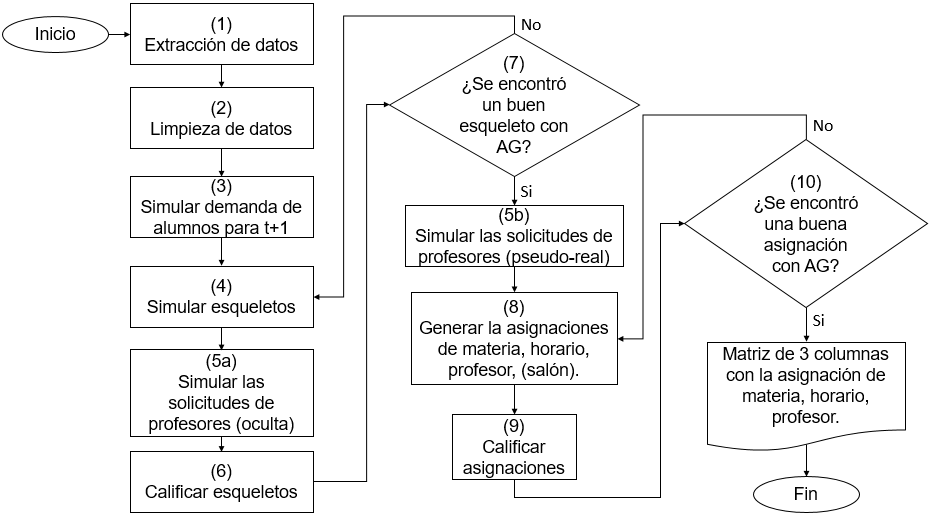
\includegraphics[width=\textwidth]{diagrama_flujo} %scale = 0.7
\caption[\textit{Diagrama de flujo de la función ``gen\_asignacion()''}]{\textit{Se muestra el diagrama de flujo de la función ``gen\_asignacion()''. Se pueden ver los pasos para obtener la matriz de asignaciones.}}\label{DF_genAsig}
\end{figure}


\section{Obtención de nombres de materias}

Antes de iniciar las simulaciones primero obtuvimos el vector \textit{vec\_nom\_materias\_total} con información de las materias encontradas en la matriz \textit{m\_grande\_total} del semestre 2008-1 al 2020-1. Dicho vector  no tiene nombres repetidos y contiene 201 materias.

En esta sección vamos a explicar cómo obtuvimos los 201 nombres de las materias que vamos a utilizar. El motivo de obtener el vector \textit{vec\_nom\_materias\_total} antes de hacer las simulaciones es para evitar problemas como el que vimos en la \figurename{~\ref{MateriaNombresDistintos}}.


***EXPLICAR LIMPIEZA DE NOMBRES DE MATERIAS***


 %%Sección %%To include subfiles in to a subfiles use \input{name_of_file}

\section{Obtención de los parámetros $q_{1}$ y $q_{2}$}

En esta sección vamos a explicar cómo obtuvimos los valores de $q_{1}$ y $q_{2}$. Son parámetros que se introducen en la función \verb@hw()@ de \textit{R}. Representan los cuantiles utilizados al calcular los intervalos de confianza. Por ejemplo si $q_{1} = 80$ entonces se calcula el intervalo al $80\%$ de confianza. Si se introducen a la función los dos parámetros entonces se calculan dos intervalos, uno al $q_{1}\%$ de confianza y el otro al $q_{2}\%$ de confianza.

Primero definimos los parámetros generales necesarios para las simulaciones:

\begin{enumerate}
\item Fijamos la semilla con \verb@set.seed(8654)@.

\item Elegimos 3 semestres para simular la demanda del número de alumnos. Los seleccionamos de los semestres que ya teníamos guardados con información real. Hicimos una comparación entre nuestros datos simulados y los reales de cada semestre. Los semestres que elegimos fueron: 2019-1, 2019-2 y 2020-1.

\item Fijamos $k = 5$ (número de semestres que se tienen como ventana de información).

\item Fijamos $num\_sim = 10$ (número de simulaciones de la demanda de alumnos para el semestre a simular).
\end{enumerate}


Después fijamos 5 materias que consideramos representativas para hacer las pruebas iniciales: \textit{Cálculo Diferencial e Integral I}, \textit{Demografía I}, \textit{Modelos no Paramétricos y de Regresión}, \textit{Administración de Riesgos Financieros} y \textit{Seminario de Investigación de Operaciones}.

Tomamos 12 posibles combinaciones de valores para $q_{1}$ y $q_{2}$, las cuales podemos ver en la \tablename{\ref{valoresQ1Q2}}. La letra \textit{L} indica que se tomó la cota inferior de $q_{1}$ y la letra \textit{U} indica que se tomó la cota superior de $q_{2}$. Con estas cotas formamos intervalos de los cuales obtuvimos las simulaciones para los 3 diferentes semestres previamente elegidos. %Con las cotas de tipo \textit{$Lq_{1}$,$Uq_{2}$} se forma un intervalo del que s

\begin{table}[H]
\centering
\begin{tabular}{|c|c|c|c|c|}
\hline 
$q_{1} \backslash q_{2}$ & 80 & 85 & 90 & 99 \\ 
\hline 
80 & - & L80,U85 & L80,U90 & L80,U99 \\ 
\hline 
85 & L85,U80 & - & L85,U90 & L85,U99 \\ 
\hline 
90 & L90,U80 & L90,U85 & - & L90,U99 \\ 
\hline 
99 & L99,U80 & L99,U85 & L99,U90 & - \\ 
\hline 
\end{tabular} 
\caption[\textit{Posibles valores para $q_{1}$ y $q_{2}$}]{\textit{Posibles valores para $q_{1}$ y $q_{2}$: Tabla que muestra todas las combinaciones de los intervalos formados con las cotas inferiores y superiores de $q_{1}$ y $q_{2}$}}\label{valoresQ1Q2}
\end{table}


Una vez hecha la simulación obtuvimos una tabla con 7 columnas: materia, intervalo, mín, media, máx, sd y seg. Donde en el renglón i se tienen los datos de la matriz de diferencias relativas de la i-ésima materia para cada intervalo de $q_{1}$ y $q_{2}$. La matriz de diferencias relativas se genera al restar, para cada materia, los datos reales menos los simulados y después dividirlos entre los reales. Por ejemplo en el primer renglón de la \figurename{\ref{matMedDispersion}} vemos que se utilizó el intervalo $(L80,U85)$ para obtener el número de alumnos simulados para el siguiente semestre de la materia \textit{Cálculo Diferencial e Integral I}. Las columnas 2, 3, 4 y 5 corresponden a las medidas de la matriz de diferencias relativas para cada materia. La última columna indica el tiempo que se tardó el proceso.

\begin{figure}[H]
\centering
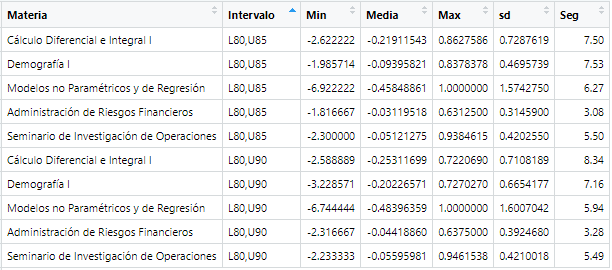
\includegraphics[scale = 0.9]{mat_med_dispersion} %width=\textwidth
\caption[\textit{Matriz con información por materia}]{\textit{Matriz con información por materia: vemos los primeros 10 renglones de la tabla obtenida con información de la matriz de diferencias relativas.}}\label{matMedDispersion}
\end{figure}


Decidimos elegir $q_{1}$ y $q_{2}$ en base a la desviación estándar. Con la \figurename{\ref{matMedDispersion}} obtuvimos una matriz de dos columnas que contine en su primer columna el intervalo y en la segunda el promedio de la desviación estándar para cada intervalo de las 5 materias. Los datos de dicha matriz los podemos ver en la \figurename{\ref{promSD_5m_12p}}.

\begin{figure}[H]
\centering
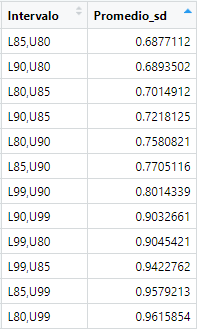
\includegraphics[scale = 1]{prom_SD_5m_12p} %width=\textwidth
\caption[\textit{Promedio de la desviación estándar: 5 materias, 12 pruebas}]{\textit{Promedio de la desviación estándar: 5 materias, 12 pruebas: Matriz con el promedio de la desviación estándar para 5 materias y 12 diferentes intervalos.}}\label{promSD_5m_12p}
\end{figure}


Los datos en la \figurename{\ref{promSD_5m_12p}} están ordenados de menor a mayor con respecto al promedio de la desviación estándar. Para la segunda prueba se eligieron los primeros 6 intervalos de dicha tabla. Se eligieron 10 materias: \textit{Álgebra Lineal I}, \textit{Álgebra Superior II}, \textit{Algoritmos Genéticos}, \textit{Análisis Matemático IV}, \textit{Análisis Numérico}, \textit{Teoría de la Medida I}, \textit{Cálculo Diferencial e Integral IV}, \textit{Graficas y Juegos}, \textit{Inglés I} y \textit{Matemáticas Actuariales para Seguro de Daños}. La tabla con el promedio de la desviación estandar de sus datos se puede ver en la \figurename{\ref{promSD_10m_6p}}.


\begin{figure}[H]
\centering
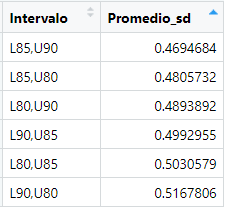
\includegraphics[scale = 1]{prom_SD_10m_6p} %width=\textwidth
\caption[\textit{Promedio de la desviación estándar: 10 materias, 6 pruebas}]{\textit{Promedio de la desviación estándar: 10 materias, 6 pruebas: Matriz con el promedio de la desviación estándar para 10 materias y 6 diferentes intervalos.}}\label{promSD_10m_6p}
\end{figure}


Para la tercera prueba elegimos, de la \figurename{\ref{promSD_10m_6p}} los intervalos que tuvieran un promedio en la desviación estándar menor a $0.5$. Seleccionamos otras 10 materias: \textit{Estadística III}, \textit{Teoría del Seguro}, \textit{Programación Entera}, \textit{Investigación de Operaciones}, \textit{Geometría Moderna I}, \textit{Geometría Analítica II}, \textit{Lógica Matemática I}, \textit{Cálculo Diferencial e Integral III}, \textit{Estadística I} y \textit{Bases de Datos}. La tabla con el promedio de la desviación estandar de sus datos se puede ver en la \figurename{\ref{promSD_10m_4p}}.


\begin{figure}[H]
\centering
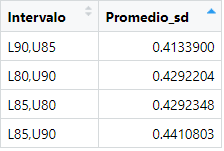
\includegraphics[scale = 1]{prom_SD_10m_4p} %width=\textwidth
\caption[\textit{Promedio de la desviación estándar: 10 materias, 4 pruebas}]{\textit{Promedio de la desviación estándar: 10 materias, 4 pruebas: Matriz con el promedio de la desviación estándar para 10 materias y 4 diferentes intervalos.}}\label{promSD_10m_4p}
\end{figure}

Podemos ver que los valores de la \figurename{\ref{promSD_10m_4p}} son muy parecidos. Hicimos una prueba con los mismos intervalos pero con 5 materias que se dan en todos los semestres y además tienen muchos alumnos. Hicimos la prueba para ver si había alguna diferencia en los datos y poder elegir un sólo intervalo. Las materias que elegimos para esta prueba fueron: \textit{Geometría Analítica I}, \textit{Cálculo Diferencial e Integral II}, \textit{Finanzas I}, \textit{Probabilidad II} y \textit{Procesos Estocásticos I}. La tabla con el promedio de la desviación estandar de sus datos se puede ver en la \figurename{\ref{promSD_5m_4p}}.


\begin{figure}[H]
\centering
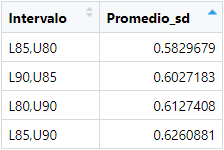
\includegraphics[scale = 1]{prom_SD_5m_4p} %width=\textwidth
\caption[\textit{Promedio de la desviación estándar: 5 materias, 4 pruebas}]{\textit{Promedio de la desviación estándar: 5 materias, 4 pruebas: Matriz con el promedio de la desviación estándar para 5 materias y 4 diferentes intervalos.}}\label{promSD_5m_4p}
\end{figure}

Analizando la información de las matrices de las Figuras \ref{promSD_10m_4p} y \ref{promSD_5m_4p}, decidimos elegir los valores de $q_{1} = 85$ y $q_{2} = 80$. Por lo que el intervalo que buscamos estará formado por la cota inferior del intervalo de confianza al $85\%$ y por la cota superior del intervalo de confianza al $80\%$. Para visualizar de una mejor manera cómo se encuentra el intervalo formado, podemos ver la \figurename{\ref{interConf}}. De ese intervalo vamos a obtener los valores para simular la demanda de alumnos.

\begin{figure}[H]
\centering
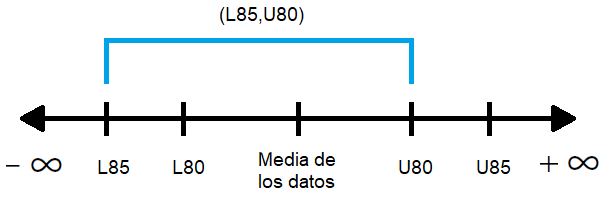
\includegraphics[scale = 0.7]{intervalos_confianza} %width=\textwidth
\caption[\textit{Diagrama de los intervalos de confianza}]{\textit{Diagrama de los intervalos de confianza: Se muestra el intervalo del que se va a obtener el número de alumnos para la simulación de cada materia en cada hora.}}\label{interConf}
\end{figure}

Finalmente con los valores de $q_{1} = 85$ y $q_{2} = 80$ hicimos una prueba aleatoria (eliminando la semilla). Las materias que elegimos para dicha prueba son: \textit{Estadística III}, \textit{Teoría del Seguro}, \textit{Cálculo Diferencial e Integral I}, \textit{Investigación de Operaciones}, \textit{Geometría Moderna I}, \textit{Geometría Analítica II}, \textit{Lógica Matemática I}, \textit{Cálculo Diferencial e Integral III}, \textit{Estadística I}, \textit{Bases de Datos}, \textit{Matemáticas Financieras}, \textit{Cálculo Diferencial e Integral II}, \textit{Probabilidad I}, \textit{Probabilidad II} y \textit{Procesos Estocásticos I}. Los resultados de la prueba aleatoria los podemos ver en la \figurename{\ref{mat_med_dispersion_pruebaAl}}. El promedio de la desviación estándar de todas las materias es $0.48$.%$0.4814898$.

\begin{figure}[H]
\centering
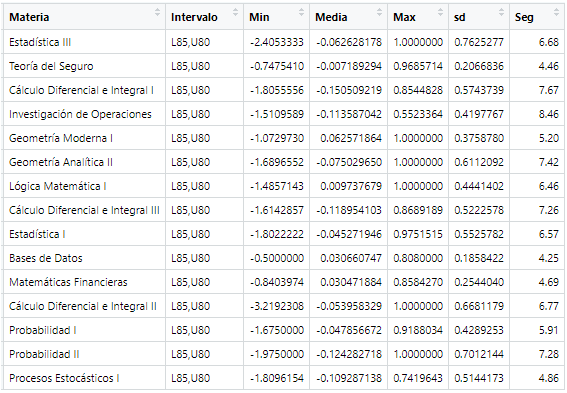
\includegraphics[scale = 0.9]{mat_med_dispersion_pruebaAleatoria} %width=\textwidth
\caption[\textit{Matriz con medidas de dispersión de prueba aleatoria}]{\textit{Matriz con medidas de dispersión de prueba aleatoria: Se muestra en cada renglón la materia y el intervalo del que se tomaron los valores para la simulación.}}\label{mat_med_dispersion_pruebaAl}
\end{figure}
 %%Sección %%To include subfiles in to a subfiles use \input{name_of_file}

\section{Obtención de nombres de profesores} \label{nomProfesores}

Antes de iniciar la simulación de las solicitudes hechas (elección de materia y de horario), primero obtuvimos información de los profesores. Guardamos dicha información en la matriz \textit{mat\_nom\_prof\_total}, la cual tiene 2 columnas. En la primer columna se tienen los nombres de todos los profesores que han impartido clase desde el semestre 2015-1 hasta el 2020-1. Dichos nombres los obtuvimos de la matriz \textit{m\_grande\_2015}. En la segunda columna de la matriz, se tiene un $1$ si el profesor es de tiempo completo y un $0$ si es de asignatura.

En las siguientes subsecciones veremos cómo llenamos la segunda columna de la matriz \textit{mat\_nom\_prof\_total} y cómo hicimos la limpieza de los nombres de los profesores.

\subsection{Profesores de tiempo completo}

Para llenar la segunda columna de la matriz \textit{mat\_nom\_prof\_total} ingresamos a la página \url{http://www.matematicas.unam.mx/index.php/nosotros/profesores-de-tiempo-completo} del Departamento de Matemáticas. Con la aplicación \textit{SelectorGadget} seleccionamos el vector con el nombre de los profesores de tiempo completo. En la \figurename{~\ref{profTC_SelectorGadget}} podemos ver el código CSS que utilizamos para obtener los datos en \textit{R}. También observamos que se seleccionaron 94 profesores.

\begin{figure}[H]
\centering
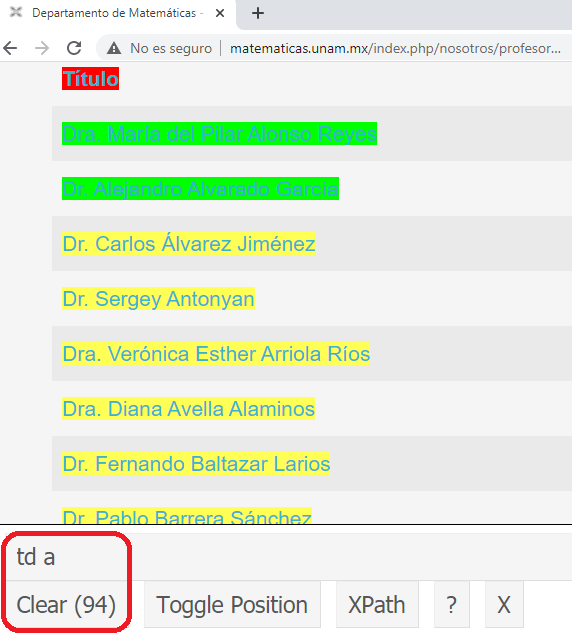
\includegraphics[scale = 0.8]{profesores_TC_SelectorGadget} %width=\textwidth
\caption[\textit{Profesores de tiempo completo: SelectorGadget}]{\textit{Profesores de tiempo completo obtenidos con la aplicación SelectorGadget: Muestra la selección de profesores de tiempo completo con la aplicación SelectorGadget. Se puede ver el código CSS utilizado en R.}}\label{profTC_SelectorGadget}
\end{figure}

Al extraer la información en \textit{R} obtuvimos un vector con 94 entradas. En la \figurename{~\ref{profTC_sinLimpiar}} podemos ver los primeros 20 valores del vector. Notamos que cada entrada del vector inicia con los caracteres $\backslash n \backslash t \backslash t \backslash t \backslash t \backslash t \backslash t \backslash t$. Estos caracteres, en la presentación final de la página de internet, indican un salto de línea y las tabulaciones o espacios que se tienen de izquierda a derecha.

\begin{figure}[H]
\centering
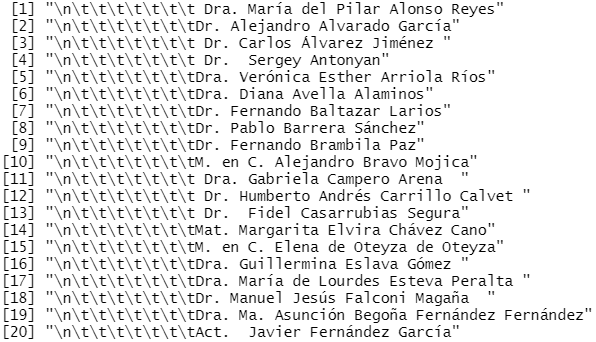
\includegraphics[scale = 0.8]{profesores_TC_sinLimpiar} %width=\textwidth
\caption[\textit{Vector de profesores de tiempo completo}]{\textit{Vector de profesores de tiempo completo: Se observan las primeras 20 entradas del vector obtenido con la aplicación SelectorGadget al dar click en un profesor de tiempo completo.}}\label{profTC_sinLimpiar}
\end{figure}

Limpiamos los datos para obtener un vector que sólo tuviera los nombres de los profesores, sin su título. Eliminamos el título porque en los horarios publicados en las páginas de la FC sus nombres no tienen título. También eliminamos los espacios finales que había en algunos nombres.

De esta manera obtuvimos el vector con el nombre de los profesores de tiempo completo del Departamento de Matemáticas. Dicho vector lo comparamos con la primer columna de la matriz \textit{mat\_nom\_prof\_total}, cuando los nombres coincidieron, pusimos un $1$ en el renglón correspondiente.

Al limpiar los datos encontramos 11 nombres que analizamos de manera particular porque no aparecía el $1$ en su respectivo renglón. Encontramos que no aparecía la información necesaria en la matriz \textit{mat\_nom\_prof\_total} por diferencias en los nombres. Encontramos diferencias por acentos, por mayúsculas y por nombres incompletos. En la \tablename{~\ref{DifNomProfTC}} vemos los nombres que aparecen en las páginas de la FC comparados con los que aparecen en la página del Departamento de Matemáticas.

\begin{table}[h]
\centering
\resizebox{\textwidth}{!}{%
  \begin{tabular}{|c|c|}
  \hline 
  \textbf{Nombre en páginas de la FC} & \textbf{Nombre en página del Depto. de Matemáticas} \\ 
  \hline 
  Alejandro Ricardo Garciadiego Dantan & Alejandro Ricardo Garciadiego Dantán \\ 
  \hline 
  Edith Corina Sáenz Valadez & Edith Corina Sáenz Valadéz \\ 
  \hline 
  Emilio Esteban Lluis Puebla & Emilio Lluis Puebla \\
  \hline 
  Guillermo Javier Francisco Sienra Loera & Guillermo Sienra Loera \\
  \hline 
  María Asunción Begoña Fernández Fernández & Ma. Asunción Begoña Fernández Fernández \\ 
  \hline 
  María Concepción Ana Luisa Solís González-Cosío & Ana Luisa Solís González Cosío \\ 
  \hline
  María Isabel Puga Espinosa & Isabel Puga Espinosa \\ 
  \hline 
  María Lourdes Velasco Arreguí & María de Lourdes Velasco Arregui \\ 
  \hline 
  Mucuy-Kak del Carmen Guevara Aguirre & Mucuy-kak del Carmen Guevara Aguirre \\ 
  \hline 
  Oscar Alfredo Palmas Velasco & Óscar Alfredo Palmas Velasco \\ 
  \hline 
  Úrsula Xiomara Iturrarán Viveros & Úrsula Iturrarán Viveros \\ 
  \hline 
  \end{tabular}
} 
\caption[\textit{Diferencias en nombres de profesores de tiempo completo}]{\textit{Diferencias en nombres de profesores de tiempo completo: Se muestran los 11 nombres de los profesores de tiempo completo que se analizaron de manera individual.}}\label{DifNomProfTC}
\end{table}

\subsection{Profesores de asignatura}

Al llenar la matriz \textit{mat\_nom\_prof\_total} con los nombres de los profesores vimos que la dimensión de dicha matriz es $1387 \times 2$. Por lo que tenemos 1387 nombres de profesores de los cuales 94 son profesores de tiempo completo. En esta subsección explicaremos cómo hicimos la limpieza de los nombres de los profesores de asginatura. Es decir los 1293 nombres que nos falta por analizar.











Algunas notas a considerar de esta matriz son:
  
  \begin{itemize}
\item[-] Hay profesores que se repiten por diferencia de acentos, como: \textit{César Alejandro Arellano Ruíz, Luis Eduardo García Hernández}.

\item[-] Hay profesores que se repiten por tener a lado el nombre de los ayudantes, como: \textit{Fermín Alberto Viniegra Heberlein, Edgar Vázquez Luis}.

\item[-] Puede haber profesores que ya no impartan clases en la FC.
\end{itemize}
 %%Sección %%To include subfiles in to a subfiles use \input{name_of_file}

\section{Simulación de tamaño de grupos} \label{SimTamGpos}

Definimos el tamaño de un grupo como el número de alumnos que tiene cada clase. Hicimos una función en \textit{R} que simula el tamaño de los grupos con respecto a los profesores. Decidimos realizar de esta manera la simulación porque queremos que el número de alumnos de cada grupo dependa de los profesores y no de la distribución general que tiene el tamaño de los grupos (ver Sección \ref{DitribTamGpos}). %Bajo el supuesto de que todos los profesores tienen cupo en sus grupos, los alumnos eligen una materia con respecto al profesor.

La función realiza los siguientes pasos (para cada uno de los profesores):
  
\begin{enumerate}
%\item Definir \textit{m\_grande\_2015} la cual es una submatriz de \textit{m\_grande\_total} con los datos de los semestres del 2015-1 al 2020-1.

\item Obtener, de \textit{m\_grande\_2015}, la información del número de alumnos que ha tenido un profesor.

\item Tomar el mínimo $(a)$ y el máximo $(b)$ de esos datos.

\item Obtener un número con la función \verb@sample(a:b, size=1)@.

\item Regresar el número obtenido en el paso anterior.
\end{enumerate}


\section{Simulación de solicitudes de profesores} \label{SimSolicitudesProfesores}

En esta sección vamos a explicar cómo hicimos la simulación de la solicitud de los profesores. En la vida real los profesores pueden elegir libremente las materias que quieren impartir y seleccionan las horas a las que desean impartir sus clases. Dado que no contamos con esa información decidimos simular la elección de materias y horarios en base a la información que tenemos de semestres anteriores.

Como vimos en la \figurename{~\ref{DF_genAsig}} simulamos dos veces las solicitudes de los profesores, en el proceso de asignación. A la primera vez que simulamos las solicitudes la llamaremos \textit{Solicitud oculta} y a la segunda la llamaremos \textit{Solicitud pseudo-real}. La explicación de su uso lo vemos a continuación.

\begin{itemize}
\item[-] Solicitud oculta: La llamamos oculta porque nos ayuda para la generación de los esqueletos. No influye directamente en la asignación final.

\item[-] Solicitud pseudo-real: Es la simulación de las posibles elecciones que los profesores harían en la vida real. Nos ayuda directamente a realizar la asignación final.
\end{itemize}

El procedimiento para ambos casos es prácticamente el mismo. Al finalizar el proceso obtuvimos una matriz, llamada \textit{mat\_1\_solicitud}, la cual tiene la información de la solicitud de un profesor. La matriz tiene 5 columnas \textit{(Profesor, TC, Materia, Num\_Materia, Horario)} y 6 renglones. Los pasos que realizamos para obtener la matriz \textit{mat\_1\_solicitud}, con la solicitud de un profesor, son los siguientes:

  \begin{enumerate}
%\item Definir \textit{m\_grande\_2015} la cual es una submatriz de \textit{m\_grande\_total} con los datos de los semestres del 2015-1 al 2020-1.

\item Llenar la columna \textit{Profesor} con el nombre del profesor del cual queremos realizar la solicitud.

\item Llenar la columna \textit{TC} dependiendo del tipo de profesor que se haya elegido en el paso anterior. Esta columna tiene un 1 en cada renglón si el profesor es de tiempo completo y un 0 si el profesor es de asignatura.

\item Obtener, de \textit{m\_grande\_2015}, la información de las materias que ha impartido el profesor elegido. Guardar la información en el vector \textit{materias\_profesor}. Se tienen 3 casos con respecto al número de materias que tiene el vector:

\begin{enumerate}
\item El número de materias es 2: Llenar los primeros 3 renglones, de la columna \textit{Materia}, con la información de la materia 1 y los últimos 3 renglones con la información de la materia 2.

\item El número de materias es mayor o igual a 3: Se toma una muestra de dos materias, con la función \verb@sample(materias_profesor, size = 2)@ en \textit{R}. Se llena la columna \textit{Materia} como el caso anterior.

\item El número de materias es 1: Llenar la columna \textit{Materia} con esa materia.
\end{enumerate}

\item Llenar la columna \textit{Num\_Materia} de \textit{mat\_1\_solicitud} con los números de materia correspondientes a las materias elegidas en el paso anterior.

\item Obtener, de \textit{m\_grande\_2015}, la información de las horas en las que ha dado clases el profesor elegido. Guardar la información en el vector \textit{horas\_profesor}. Se tienen 4 casos con respecto al número de horas que se encuentran en el vector:

\begin{enumerate}
\item El número de horas es 3: Llenar los renglones 1 y 4, de la columna \textit{Horario}, con la información de la hora 1; los renglones 2 y 5 con la información de la hora 2 y los renglones 3 y 6 con la información de la hora 3.

\item El número de horas es mayor o igual a 4: Se toma una muestra de 3 horas, con la función \verb@sample(horas_profesor, size = 3)@ en \textit{R}. Se llena la columna \textit{Horario} como el caso anterior.

\item El número de horas es 2: Llenar los renglones 1,2,4 y 5, de la columna \textit{Horario}, con la información de la hora 1 y los renglones 3 y 6 con la información de la hora 2.

\item El número de horas es 1: Llenar la columna \textit{Horario} con esa hora.
\end{enumerate}
\end{enumerate}

En la \figurename{~\ref{mat_1_solicitud_Margarita}} vemos un ejemplo de la matriz \textit{mat\_1\_solicitud}.

\begin{figure}[H]
\centering
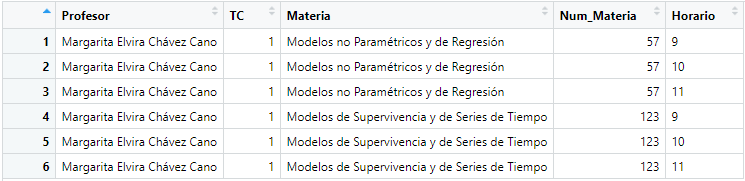
\includegraphics[width=\textwidth]{mat_1_solicitud_Margarita} %scale = 0.8
\caption[\textit{Ejemplo de matriz de solicitudes de un profesor}]{\textit{Ejemplo de matriz de solicitudes de un profesor: Se observa un ejemplo de la matriz mat\_1\_solicitud para un profesor de tiempo completo.}}\label{mat_1_solicitud_Margarita}
\end{figure}

El proceso se repite para cada uno de los profesores en la matriz \textit{mat\_nom\_prof\_total} obtenida en la Sección \ref{nomProfesores}. La matriz formada con las solicitudes de todos los profesores la llamamos \textit{mat\_solicitudes}. A ella le quitamos los renglones repetidos. Con estos pasos realizamos la \textit{Solicitud oculta}. Ésta nos sirve para poder simular adecuadamente los esqueletos.

Para realizar la \textit{Solicitud pseudo-real} hacemos una comparación del esqueleto generado y la matriz \textit{mat\_solicitudes}. Cabe señalar que la \textit{Solicitud pseudo-real} depende del esqueleto simulado y la \textit{Solicitud oculta} no.
 %%Sección %%To include subfiles in to a subfiles use \input{name_of_file}

\section{Simulación de la demanda de alumnos} \label{SimDemandaAlumnos}

La demanda del número de alumnos para el siguiente semestre la hicimos por materia y por hora. Para poder realizar la simulación lo primero que hicimos fue acomodar la información que teníamos por semestres y por hora. El procedimiento que seguimos fue el siguiente:
  
  \begin{enumerate}
\item Definir el semestre del cual se quiere obtener la simulación (\textit{sem\_sig}).

\item Definir el número de semestres que se quieren como ventana de información (\textit{k}).

\item Tomar una submatriz de \textit{m\_grande\_total} con la información de una materia para los semestres en la ventana de información.

\item Para cada semestre dentro de la ventana de información se suma el número de alumnos en cada hora.

\item Se obtiene una matriz de $t \times k$ como la que se puede ver en la \figurename{~\ref{matAl_corregidos}}. Recordemos que $t = 15$ y representa el número de horas en las que se imparten clases.
\end{enumerate}

\begin{figure}[h]
\centering
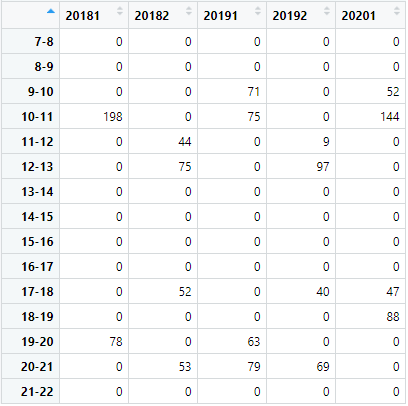
\includegraphics[scale = 0.8]{mat_alumnos_corregidos_EstadisticaIII} %width=\textwidth
\caption[\textit{Ejemplo de matriz con alumnos corregidos}]{\textit{Se puede ver la información del número de alumnos reales de la materia ``Modelos de Supervivencia y Series de Tiempo'' por semestre y por hora.}}\label{matAl_corregidos}
\end{figure}

%Con el procedimiento descrito pudimos generar vectores por hora. Aplicamos la función \verb@hw()@ en \textit{R} para obtener la demanda de alumnos esperados para el siguiente semestre. En la \figurename{~\ref{vec_alum_sim}} vemos el vector con la demanda de alumnos simulados para el semestre 2020-2 de la materia \textit{Modelos de Supervivencia y Series de Tiempo}.

Con el procedimiento descrito pudimos generar vectores por hora. Aplicamos la función \verb@hw()@ en \textit{R} para obtener la demanda de alumnos esperados para el siguiente semestre. En la \figurename{~\ref{matAl_corregidos_y_sim}} vemos la matriz vista en la \figurename{~\ref{matAl_corregidos}} junto con el vector de alumnos simulados (señalado en rojo). El vector contiene la demanda de alumnos simulados para el semestre 2020-2 de la materia \textit{Modelos de Supervivencia y Series de Tiempo}.

Notamos que el valor de la demanda de alumnos es cero cuando en todos los semestres de alguna hora no hay datos. En el ejemplo, es el caso de las 7hrs, 8hrs, 13hrs, 14hrs, 15hrs, 16hrs y 21hrs.

Observando los datos de las 10hrs. vemos que en los semestres pares no hay alumnos, por lo que en la simulación se obtiene únicamente un alumno. Si vemos los datos de las 17hrs vemos que de los 5 semestres en la ventana se tienen alumnos en los semestres pares y en un semestre impar, el número de alumnos simulados para esa hora son 31 alumnos.

Con estos ejemplos podemos ver de manera tangible que el modelo respeta la estacionalidad semestral que tienen los datos.

\begin{figure}[H]
\centering
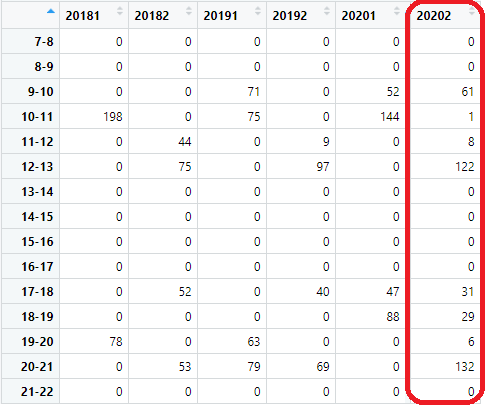
\includegraphics[scale = 0.8]{mat_alumnos_corregidos_con_Sim_EstadisticaIII} %width=\textwidth
\caption[\textit{Ejemplo de vector con demanda simulada para el 2020-2 de ``Modelos de Supervivencia y Series de Tiempo''}]{\textit{En esta figura se señala en rojo el vector con la demanda simulada para el 2020-2 de la materia ``Modelos de Supervivencia y Series de Tiempo''.}}\label{matAl_corregidos_y_sim}
\end{figure}

%\begin{figure}[H]
%\centering
%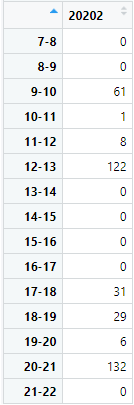
\includegraphics[scale = 0.8]{vec_alum_sim_EstadisticaIII} %width=\textwidth
%\caption[\textit{Ejemplo de vector con demanda simulada para el 2020-2 de ``Modelos de Supervivencia y Series de Tiempo''}]{\textit{Ejemplo de vector con demanda simulada para el 2020-2 de ``Modelos de Supervivencia y Series de Tiempo'': Vemos el vector con el número de alumnos simulados para el 2020-2 de la materia ``Modelos de Supervivencia y Series de Tiempo''}}\label{vec_alum_sim}
%\end{figure}

Obtuvimos vectores con la demanda simulada para cada una de las materias y formamos una matriz de $t \times m$, llamada \textit{mat\_demanda\_alumnos}. Recordemos que $m$ es el número de materias que se van a impartir. En la \figurename{~\ref{matDemandaAlum}} podemos ver un ejemplo de cómo se ve la matriz formada.

Analicemos 2 pares de grupos, primero veamos la columna de \textit{Álgebra Superior II} (2) y la de \textit{Geometría Analítica I} (4). Ambas son materias obligatorias para Actuaría, Matemáticas y Matemáticas Aplicadas. La primera corresponde a semestres pares y la segunda a semestres impares. Notamos que para \textit{Geometría Analítica I}, se tienen alumnos prácticamente en cada hora, pero el número no es muy grande. Para \textit{Álgebra Superior II} hay varias horas con cero alumnos simulados pero hay dos grandes cantidades, una a las 9hrs con 832 alumnos y la otra a las 18hrs con 224 alumnos. Con esta comparación podemos ejemplificar la diferencia entre una materia que corresponde a semestres pares y una de semestres impares.

Ahora analicemos las columnas de \textit{Seminario de Topología A} (3) y \textit{Probabilidad II} (6). La primera es una materia optativa para Matemáticas. La segunda es una materia obligatoria para Actuaría, correspondiente a semestres pares y optativa para Ciencias de la Computación, Matemáticas y Matemáticas Aplicadas. El número total de alumnos simulados para \textit{Seminario de Topología A} es menor a 20, en cambio para \textit{Probabilidad II} se tiene una gran cantidad de alumnos a las 8hrs, 9hrs y 10hrs. Considerando los valores que se tienen en el turno vespertino para \textit{Probabilidad II}, notamos que a las 19hrs también hay una gran cantidad de alumnos. Con esta comparación podemos ejemplificar la diferencia entre una materia obligatoria y una optativa, así como la diferencia entre el turno matutino y vespertino.


\begin{figure}[H]
\centering
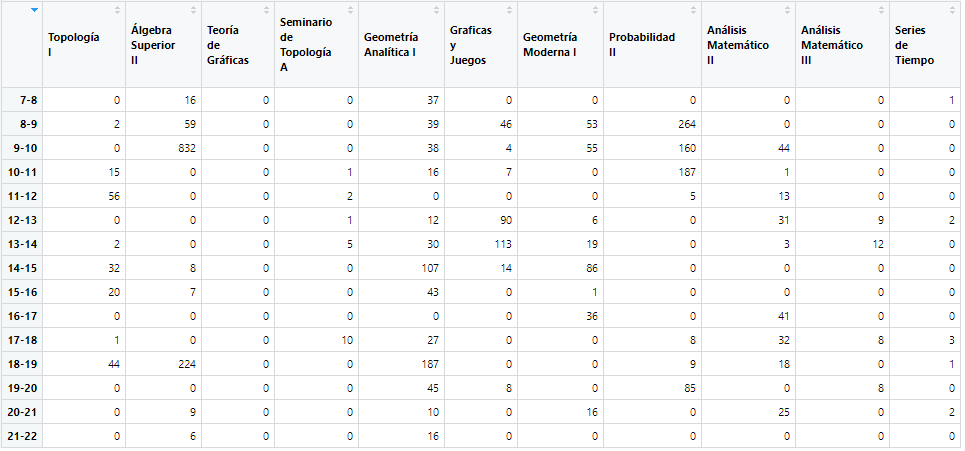
\includegraphics[scale = 0.8]{mat_demanda_alumnos} %width=\textwidth
\caption[\textit{Ejemplo de matriz con demanda simulada para el 2020-2}]{\textit{Se muestra una submatriz de ``mat\_demanda\_alumnos''. Los vectores contienen el número de alumnos simulados para el semestre 2020-2 por hora de algunas materias.}}\label{matDemandaAlum}
\end{figure}


\section{Modelo de Mezcla Gaussiana} \label{sec_GMM}

El modelo de Mezcla Gaussiana también es llamado modelo de mezcla de normales. En él se tienen dos o más distribuciones normales. Se hace una combinación lineal de ellas y se obtiene una nueva distribución de probabilidad.

En \textit{R} se puede obtener dicha distribución con la función \verb@normalmixEM()@. La función regresa un objeto de tipo \textit{mixEM} el cual contiene el modelo de una mezcla de distribuciones normales obtenidas por el algoritmo de maximización de la esperanza (EM - \textit{expectation maximization algorithm}).

Do Chuong y Batzoglou nos indican, en su artículo \textit{What is the expectation maximization algorithm?} [\ref{ChuongBatzoglou}], que el algoritmo EM es una generalización natural de la estimación por máxima verosimilitud. Ésto para el caso en donde se tiene información incompleta. Recordemos que la máxima verosimilitud se utiliza para encontrar la mejor manera de ajustar una distribución a los datos.

En el algoritmo EM, los parámetros iniciales se toman de los datos reales. Con ellos se obtienen unos parámetros finales que se convierten en los parámetros para la siguiente iteración. Así sucesivamente.

Cabe mencionar que el objeto de tipo \textit{mixEM} contiene los valores de $\mu$ y $\sigma$ finales. Éstos nos sirven para simular números aleatorios con una distribución normal. Dicha distribución tiene $k$ medias, así como $k$ desviaciones estándar. Los principales parámetros que recibe la función \verb@normalmixEM()@ son: 

\begin{itemize}
\item[-] \textit{x: } Vector con los datos a los que se les quiere aplicar el modelo.

\item[-] \textit{mu: } Vector con las medias iniciales para el algoritmo EM.

\item[-] \textit{sigma: } Vector con las desviaciones estándar iniciales del modelo.

\item[-] \textit{k: } Número de distribuciones normales que se ajustan a los datos.
\end{itemize}

En la \figurename{~\ref{GMM_alum_ini}} se puede ver el histograma con el número de alumnos esperados por hora. Los datos corresponden a una matriz \textit{mat\_demanda\_alumnos} (ver Sección \ref{SimDemandaAlumnos}). Con el comando \verb@mixmdl_1_D <- normalmixEM(wait_alumnos,k = 4)@ guardamos el modelo inicial. La línea azul de dicha figura corresponde a la densidad ajustada de 1000 números aleatorios con una distribución normal con 4 medias. El comando para obtener la densidad es: \verb@density(rnorm(1000,mean = mixmdl_1_D$mu,sd = mixmdl_1_D$sigma)@. Se tomaron los valores de $\mu$ y $\sigma$ arrojados por el modelo \textit{mixmdl\_1\_D}.

\begin{figure}[h]
\centering
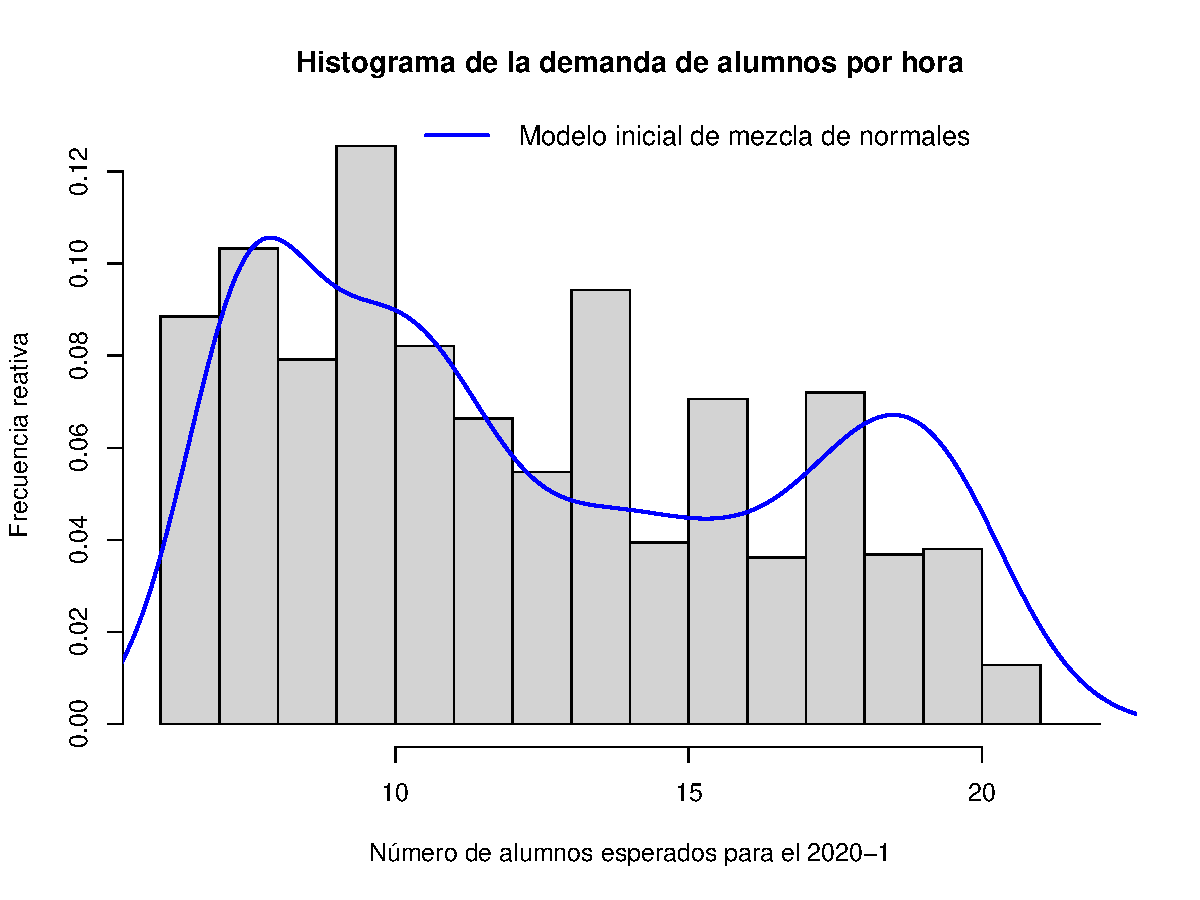
\includegraphics[scale = 0.65]{gmm_alum_ini.pdf} %width=\textwidth
\caption[\textit{Histograma del número de alumnos esperados por hora: Modelo inicial de mezcla de normales}]{\textit{Se muestra el histograma del número de alumnos esperados por hora. La línea azul corresponde a la densidad ajustada de 1000 números aleatorios con la distribución obtenida con el modelo inicial de mezcla de normales.}}\label{GMM_alum_ini}
\end{figure}

En la \figurename{~\ref{GMM_alum_fin}} se puede observar el histograma con el número de alumnos esperados por hora. Los datos corresponden a 5 matrices \textit{mat\_demanda\_alumnos} (ver Sección \ref{SimDemandaAlumnos}). Con el comando \verb@mixmdl_D <- normalmixEM(wait_alumnos_final,mixmdl_1_D$mu)@ guardamos el modelo final. En este caso la función recibió los datos del modelo inicial. Los valores de $\mu$ son: $7.49, 10.30, 13.78, 17.23$. Para obtener la densidad ajustada, mostrada en la figura (línea azul), utilizamos los valores de $\mu$ y $\sigma$ arrojados por el modelo \textit{mixmdl\_D}.

Notamos que la densidad se ajusta mejor a los datos. Ésto debido a que para este caso se tienen mejores valores iniciales. Se puede ver el pico de las 10hrs, también se observa que se toman en cuenta los picos de las 14hrs, 16hrs y 18hrs.

\begin{figure}[H]
\centering
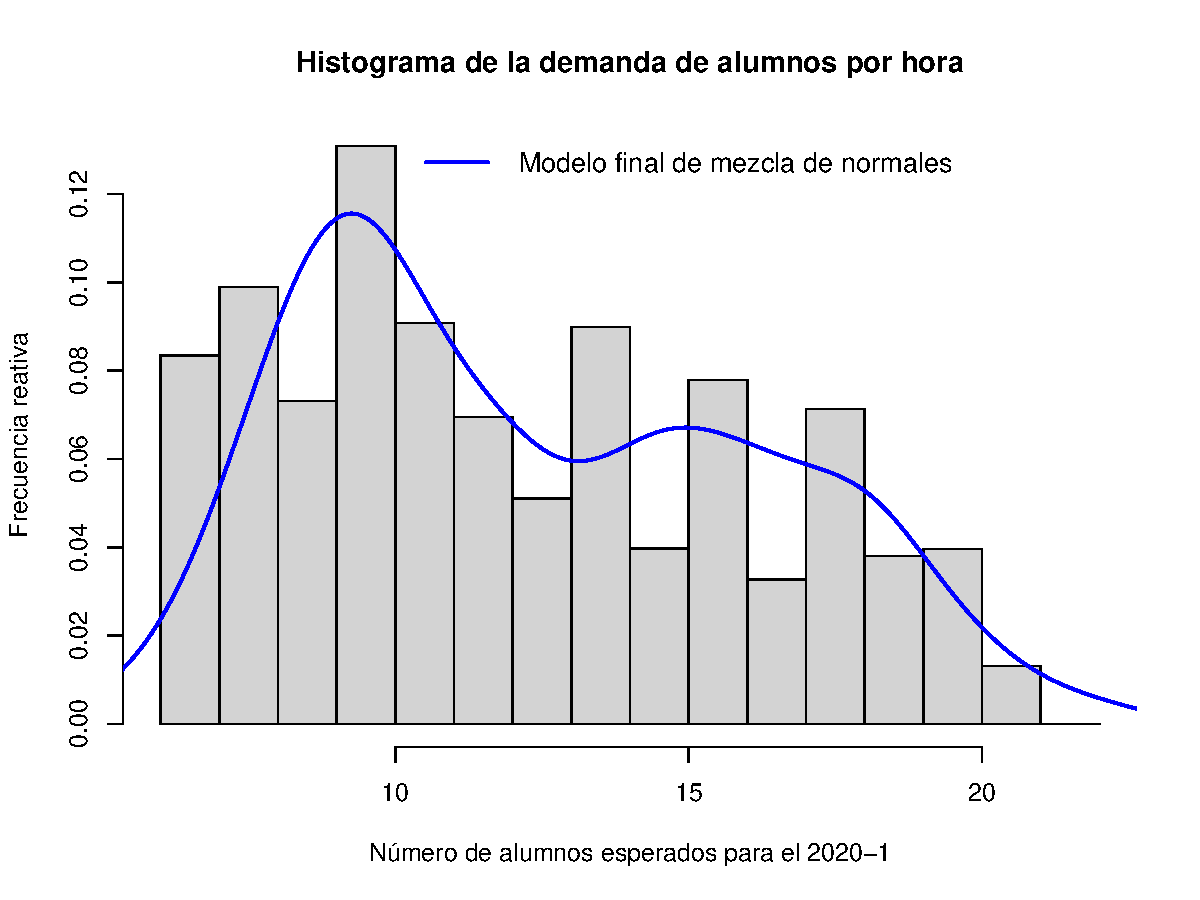
\includegraphics[scale = 0.65]{gmm_alum_fin.pdf} %width=\textwidth
\caption[\textit{Histograma del número de alumnos esperados por hora: Modelo final de mezcla de normales}]{\textit{Se muestra el histograma del número de alumnos esperados por hora. La línea azul corresponde a la densidad ajustada de 1000 números aleatorios con la distribución obtenida con el modelo final de mezcla de normales.}}\label{GMM_alum_fin}
\end{figure}


%En la \figurename{~\ref{GMM_ini_fin}} se pueden ver dos histogramas con el número de alumnos esperados por hora.
%\begin{figure}[H]
%\centering
%\subfigure[\textit{Modelo inicial}]{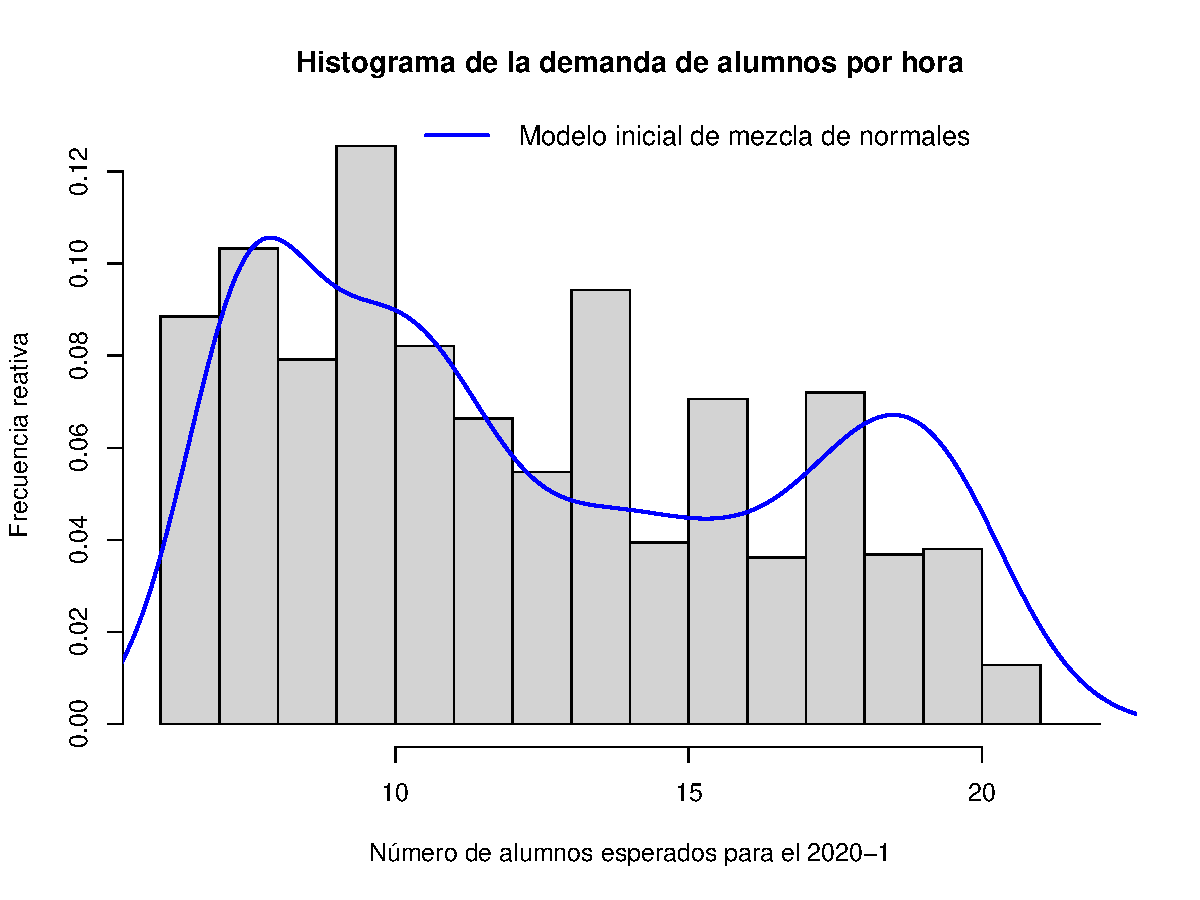
\includegraphics[width=12cm]{gmm_alum_ini.pdf}} %%Ping\"uino %%[angle=30]
%	\subfigure[\textit{Modelo final}]{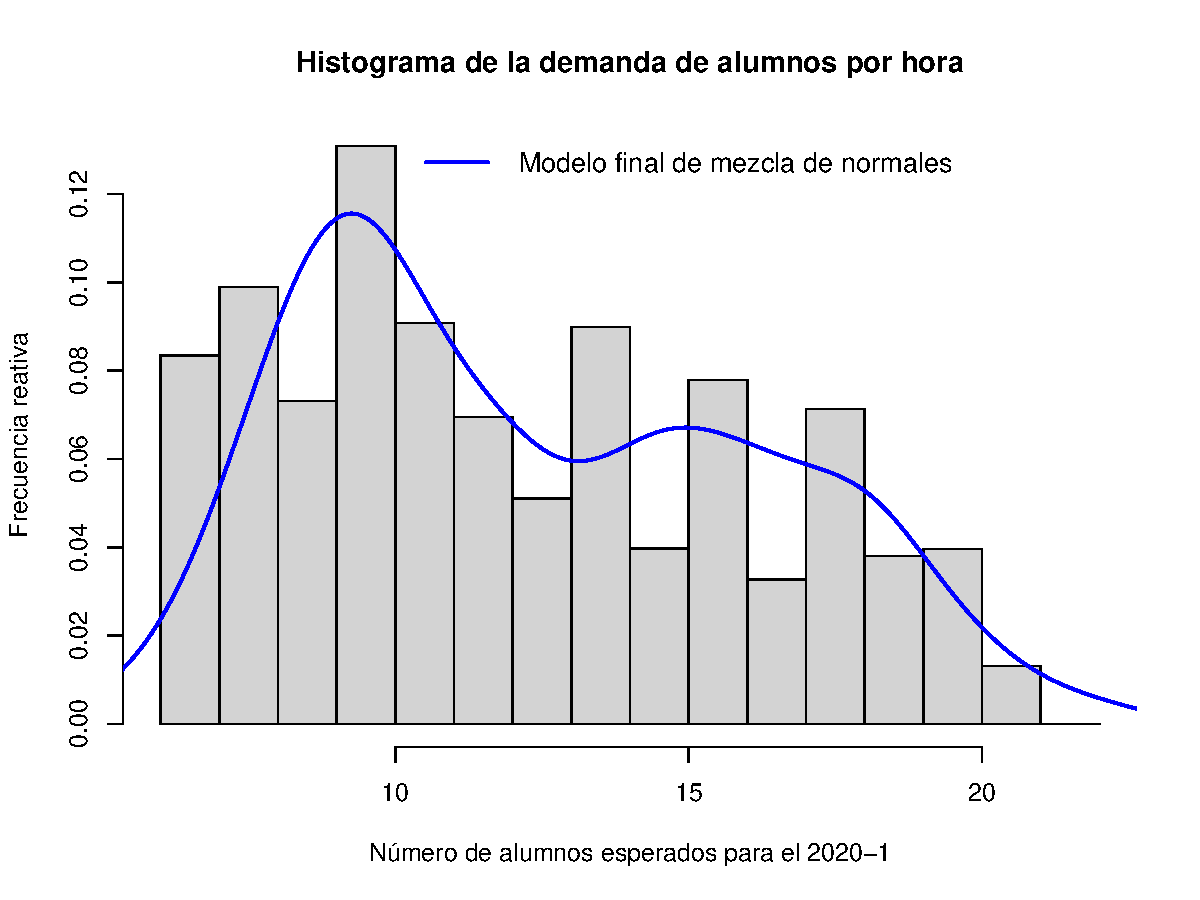
\includegraphics[width=12cm]{gmm_alum_fin.pdf}}
%	\caption[\textit{Histogramas con el número de alumnos esperados por hora}]{\textit{Se muestran dos histogramas con el número de alumnos esperados por hora. Cada uno tiene la densidad ajustada de 1000 números aleatorios con la distribución obtenida con el modelo de mezcla de normales.}}\label{GMM_ini_fin}
%\end{figure}


%En la \figurename{~\ref{GMM_inicial_final}} se muestran dos histogramas con los datos iniciales y finales, respectivamente. Las líneas verdes corresponden al ajuste con la función \verb@density()@ en \textit{R} y las azules al modelo de mezcla de normales.
%
%\begin{figure}[H]
%\centering
%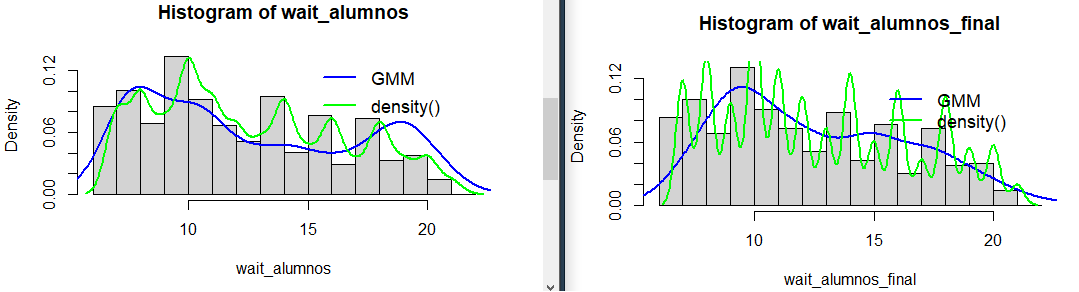
\includegraphics[width=\textwidth]{histograma_y_GMM} %scale = 1
%\caption{\textit{Mezcla de normales inicial y final}}\label{GMM_inicial_final}
%\end{figure}

%\url{https://www.youtube.com/watch?v=REypj2sy_5U&ab_channel=VictorLavrenko}
%
%\url{https://www.youtube.com/watch?v=iQoXFmbXRJA&ab_channel=VictorLavrenko}
%
%\url{https://www.youtube.com/watch?v=pYxNSUDSFH4&ab_channel=StatQuestwithJoshStarmer}
%
%\url{https://www.youtube.com/watch?v=XepXtl9YKwc&ab_channel=StatQuestwithJoshStarmer} %%  The goal of the maximum likelihood is to find the optimal way to fit a distribution to the data.
%
%\url{https://www.youtube.com/watch?v=s3sTSA_GXV8&ab_channel=InstitutodeInformaticaUACh}
%
%\url{https://www.youtube.com/watch?v=_igVkRP9TFE&ab_channel=InstitutodeInformaticaUACh}
%
%\url{https://natureofcode.com/book/chapter-9-the-evolution-of-code/}



%\begin{figure}[H]
%\centering
%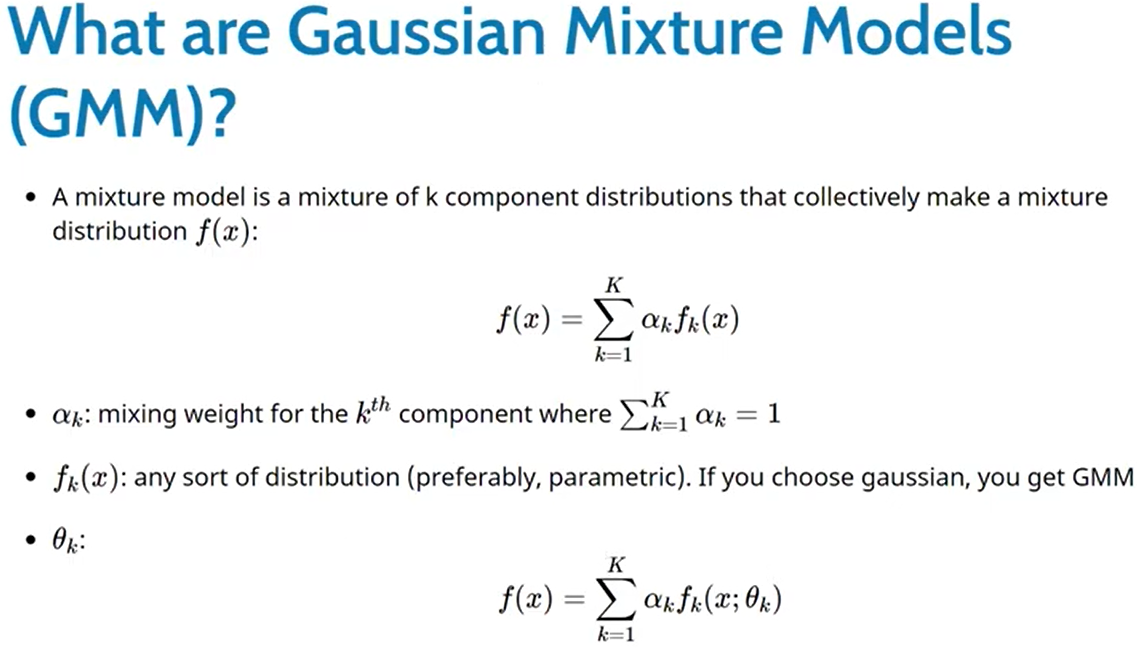
\includegraphics[scale = 0.5]{GMM_1} %width=\textwidth
%\caption{\textit{GMM 1}}
%\end{figure}
%
%\begin{figure}[H]
%\centering
%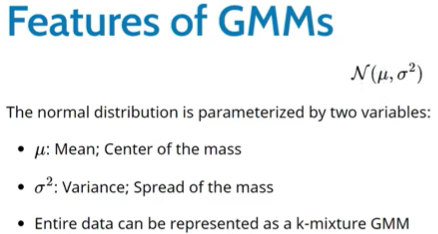
\includegraphics[scale = 0.5]{GMM_2} %width=\textwidth
%\caption{\textit{GMM 2}}
%\end{figure}
%
%\begin{figure}[H]
%\centering
%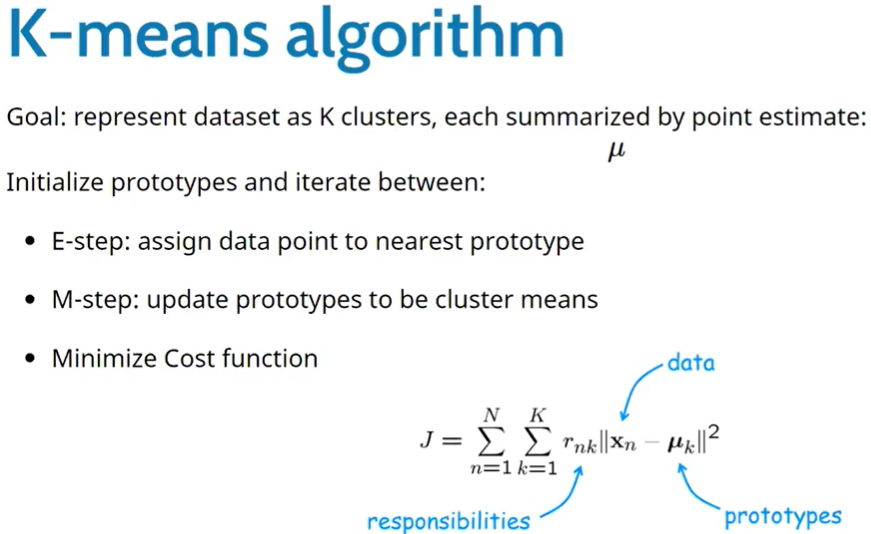
\includegraphics[scale = 0.5]{GMM_3} %width=\textwidth
%\caption{\textit{GMM 3}}
%\end{figure}
%
%\begin{figure}[H]
%\centering
%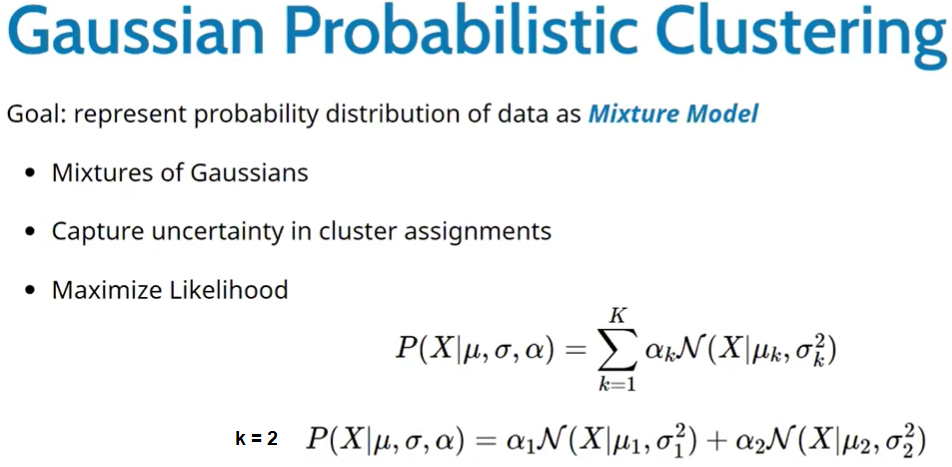
\includegraphics[scale = 0.5]{GMM_4} %width=\textwidth
%\caption{\textit{GMM 4}}
%\end{figure}
%
%\begin{figure}[H]
%\centering
%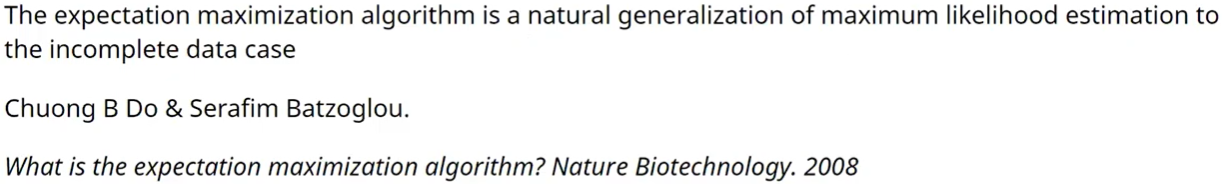
\includegraphics[scale = 0.5]{GMM_5} %width=\textwidth
%\caption{\textit{GMM 5}}
%\end{figure}
%
%\begin{figure}[H]
%\centering
%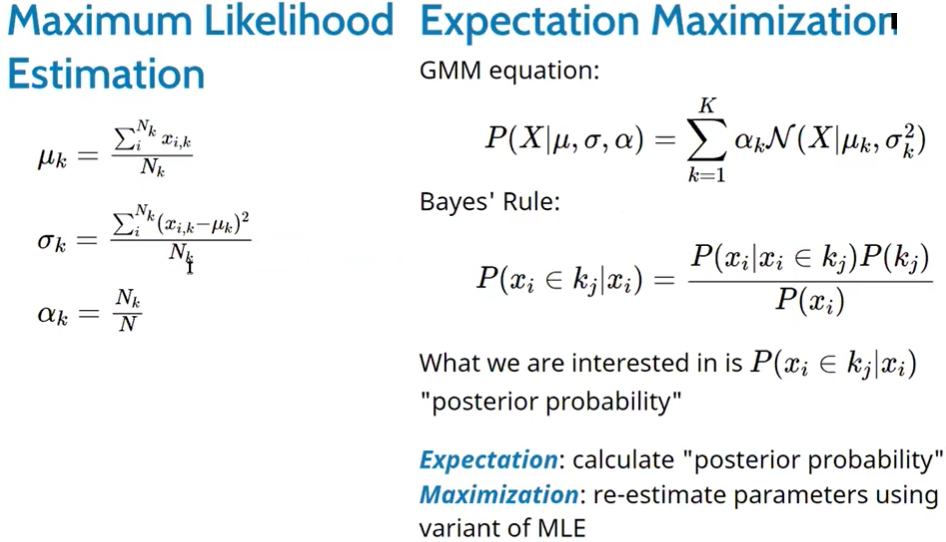
\includegraphics[scale = 0.5]{GMM_6} %width=\textwidth
%\caption{\textit{GMM 6}}
%\end{figure}
%
%\begin{figure}[H]
%\centering
%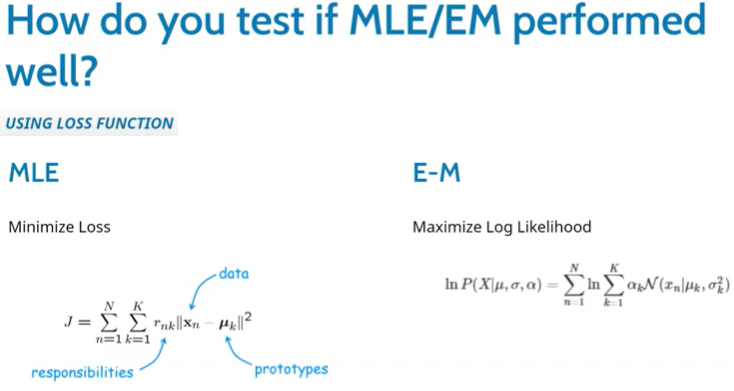
\includegraphics[scale = 0.5]{GMM_7} %width=\textwidth
%\caption{\textit{GMM 7}}
%\end{figure}

El modelo de mezcla de normales lo utilizamos para simular los esqueletos de los horarios. En las siguientes secciones veremos cómo aplicamos la función \verb@normalmixEM()@ para obtener la matriz \textit{mat\_esqueleto}.


\section{Obtención de $D'$ y $D_{0}$} \label{GMM_D}

Los esqueletos que vamos a simular dependen de la demanda de alumnos. En esta sección vamos a mostrar 4 diferentes metodologías que probamos para poder simular adecuadamente los esqueletos. Ésto basándonos en el número de alumnos simulados para el siguiente semestre. %Al final de esta sección, vamos a describir el método con el que generamos la matriz \textit{mat\_esqueleto}.


Definimos las siguientes matrices:

\begin{itemize}
\item[-] $D': $ Matriz de $t \times m$, con la demanda simulada por alguna de las 4 metodologías.

\item[-] $D^{0}: $ Matriz de $t \times m$, con la cual se va a comparar $D'$ para calificarla. Esta matriz se obtiene haciendo el promedio entre una matriz \textit{mat\_demanda\_alumnos} (ver Sección \ref{SimDemandaAlumnos}) y una matriz de demanda de alumnos, obtenida con el modelo de mezcla de normales (ver Sección \ref{sec_GMM}).
\end{itemize}

La calificación de las metodologías depende de la diferencia relativa entre $D^{0}$ y $D'$. Los pasos que seguimos para obtener las calificiones son:

\begin{enumerate}
\item Definir la matriz $C$, de $t \times m$. Esta matriz va a guardar las calificaciones por grupo de $D'$.

\item Para cada $C_{h,j}$ guardar el valor de $\dfrac{D_{h,j}^{0} - D'_{h,j}}{D_{h,j}^{0}}$. 

\item Si $D_{h,j}^{0} = 0$ entonces $C_{h,j} = 1$ si faltan alumnos y $C_{h,j} = -1$ si sobran alumnos, es decir: $C_{h,j} = \left \{ \begin{matrix} 1 & \mbox{si }D_{h,j}^{0} > D'_{h,j}\\ 
-1 & \mbox{si }D_{h,j}^{0} < D'_{h,j}\\ 0 & \mbox{e.o.c. }\end{matrix}\right.$



\item Definir el vector \textit{vec\_calif\_x\_materia} con el promedio por columna de $C$. Este vector guarda las calificaciones por materia de $D'$.
\end{enumerate}

Para cada metodología, realizamos 10 simulaciones y calificamos las matrices $D'$ generadas. Con este procedimiento obtuvimos 4 matrices de 10 renglones y $m$ columnas. Graficamos cada matriz con la función \verb@matplot()@ en \textit{R}. Cada gráfica contiene $m$ líneas con 10 puntos cada línea. A continuación mostramos las 4 gráficas.

En la \figurename{~\ref{fig_metodo_A}} vemos las calificaciones por materia de la metodología A. Notamos que se encuentran entre -5 y 1. Ésto quiere decir que en promedio con este método sobra hasta un 500\% de alumnos y falta casi un 100\% al hacer la simulación.

\begin{figure}[H]
\centering
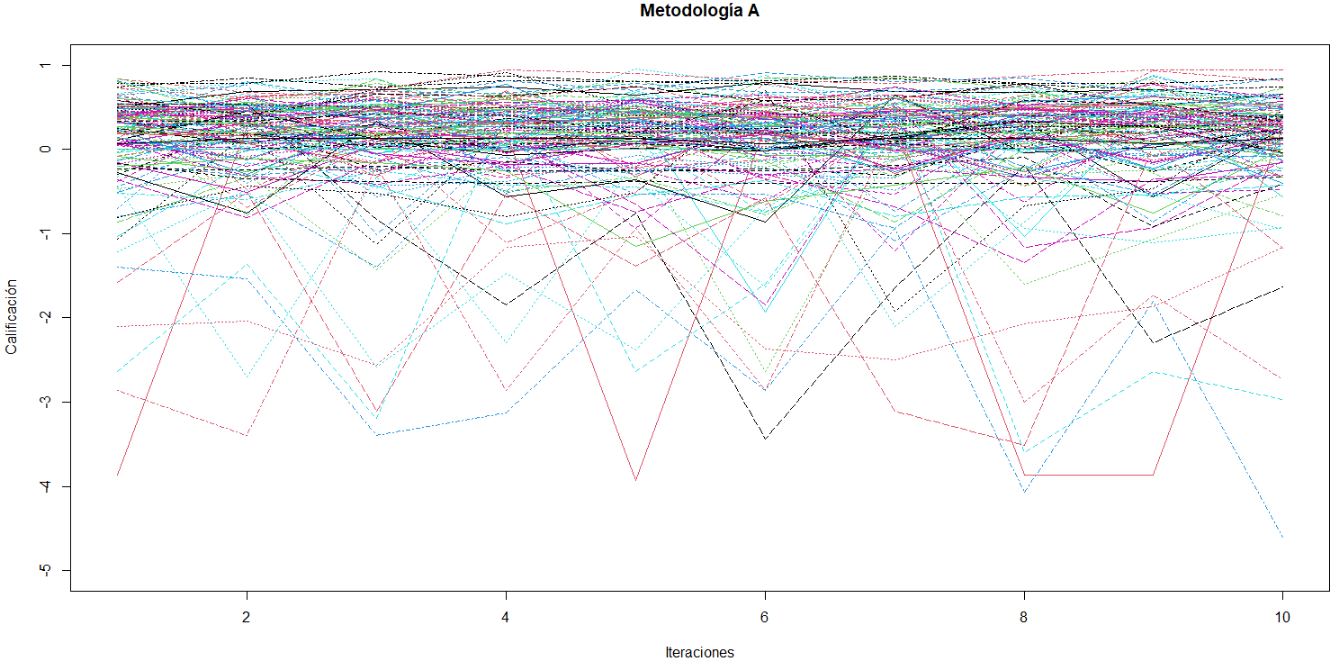
\includegraphics[width=\textwidth]{calif3_escala_metodo_A} %scale = 0.7
\caption[\textit{Metodología A}]{\textit{Se muestran las calificaciones por materia de la metodología A.}}\label{fig_metodo_A}
\end{figure} 


En la \figurename{~\ref{fig_metodo_B}} vemos las calificaciones por materia de la metodología B. Notamos que se encuentran entre -0.5 y 0.8. Ésto quiere decir que en promedio con este método sobra hasta un 50\% de alumnos y falta casi un 80\% al hacer la simulación.

\begin{figure}[H]
\centering
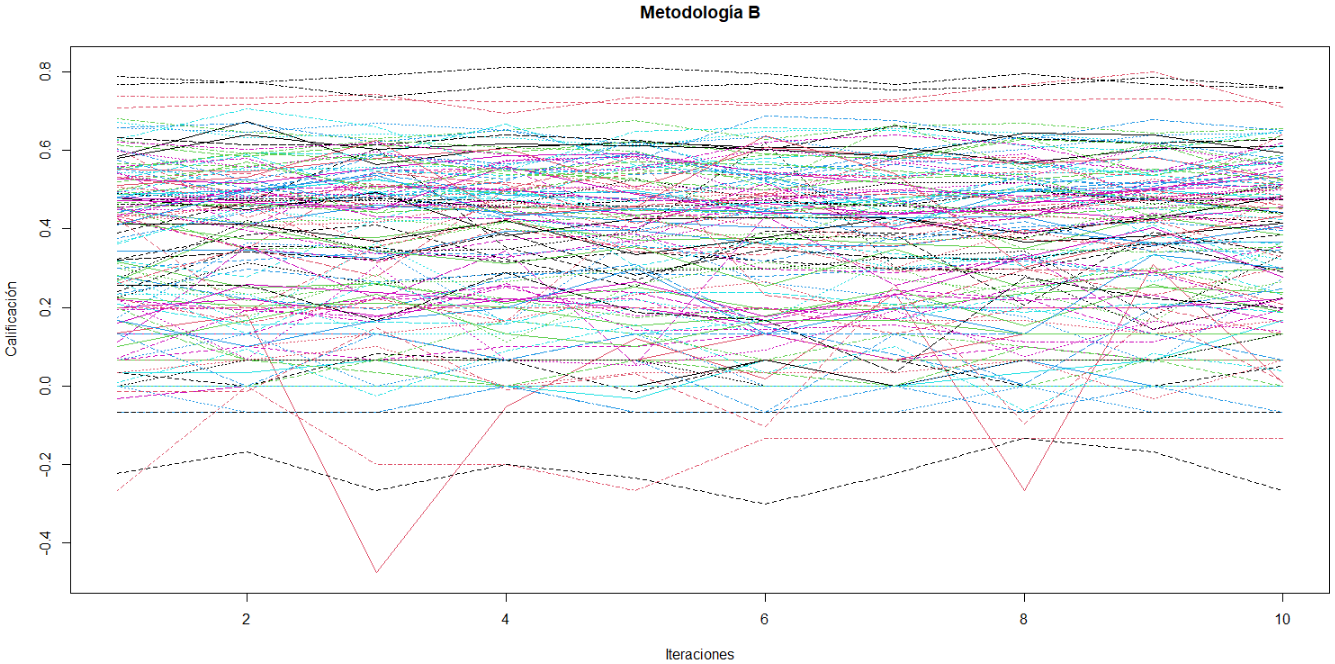
\includegraphics[width=\textwidth]{calif3_metodo_B} %scale = 0.7
\caption[\textit{Metodología B}]{\textit{Se muestran las calificaciones por materia de la metodología B.}}\label{fig_metodo_B}
\end{figure} 


En la \figurename{~\ref{fig_metodo_C}} vemos las calificaciones por materia de la metodología C. Notamos que, al igual que en la metodología B, las calificaciones se encuentran entre -0.5 y 0.8. En este caso observamos que hay una mayor concentración de materias (líneas) entre 0.5 y 0.8. Ésto comparado con el método B que tiene una mayor concentración entre 0.4 y 0.6.

\begin{figure}[H]
\centering
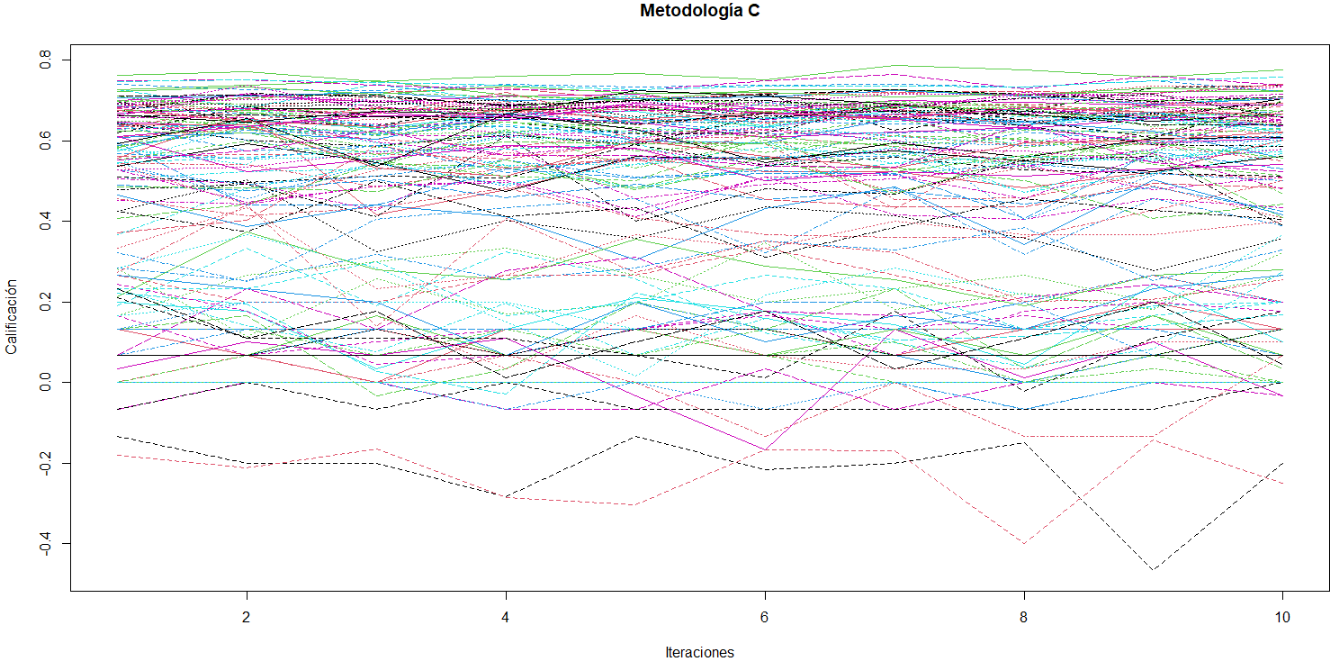
\includegraphics[width=\textwidth]{calif3_metodo_C} %scale = 0.7
\caption[\textit{Metodología C}]{\textit{Se muestran las calificaciones por materia de la metodología C.}}\label{fig_metodo_C}
\end{figure}


En la \figurename{~\ref{fig_metodo_D}} vemos las calificaciones por materia de la metodología D. Notamos que se encuentran entre -6 y 0.4. Ésto quiere decir que en promedio con este método sobra hasta un 600\% de alumnos y falta casi un 40\% al hacer la simulación. Podemos observar que sólo una materia tiene calificaciones por debajo de -3. En general todas se concentran entre -2.5 y 0.4.

\begin{figure}[H]
\centering
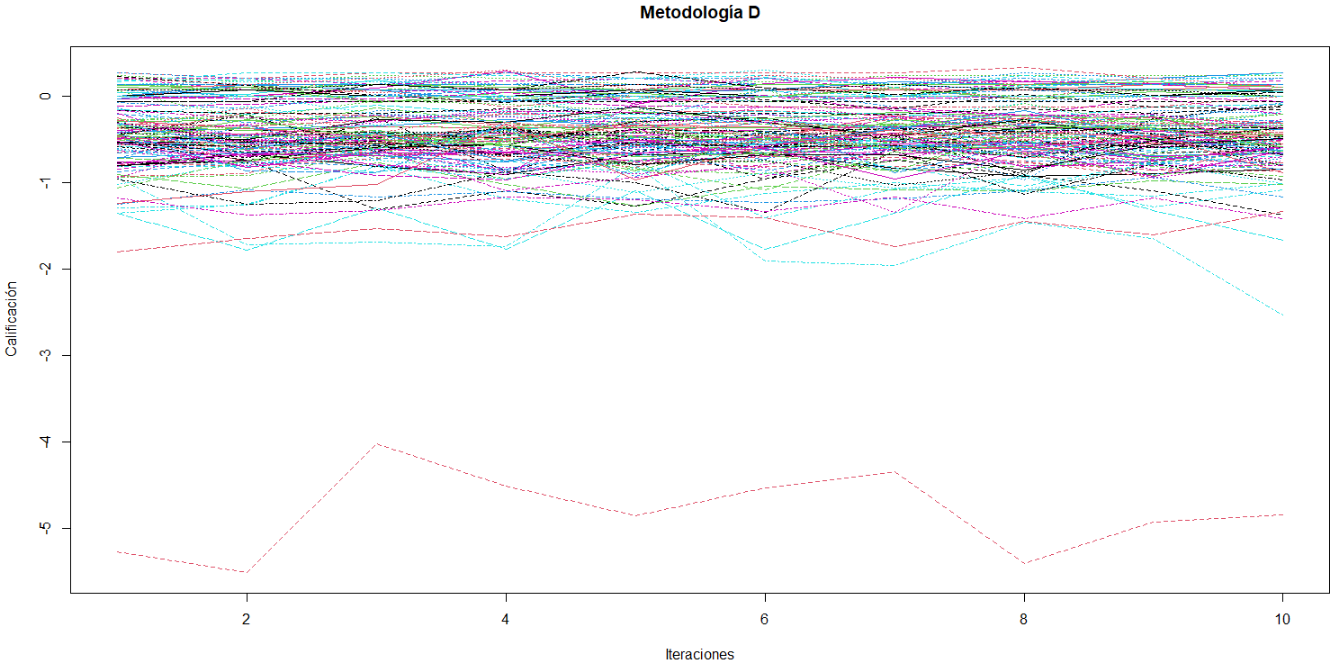
\includegraphics[width=\textwidth]{calif3_metodo_D} %scale = 0.7
\caption[\textit{Metodología D}]{\textit{Se muestran las calificaciones por materia de la metodología D.}}\label{fig_metodo_D}
\end{figure} 


Decidimos analizar las metodologías $B$ y $C$ ya que son las que muestran las mejores calificaciones. Para ello graficamos las matrices de calificaciones con la función \verb@heatmap()@ en \textit{R}. Cabe aclarar que las matrices de calificaciones están ordenadas de menor a mayor por renglones. En la \figurename{~\ref{fig_heatmap_B}} vemos el correspondiente a la metodología $B$. En la \figurename{~\ref{fig_heatmap_C}} vemos el \textit{heatmap} referente a la metodología $C$.

\begin{figure}[H]
\centering
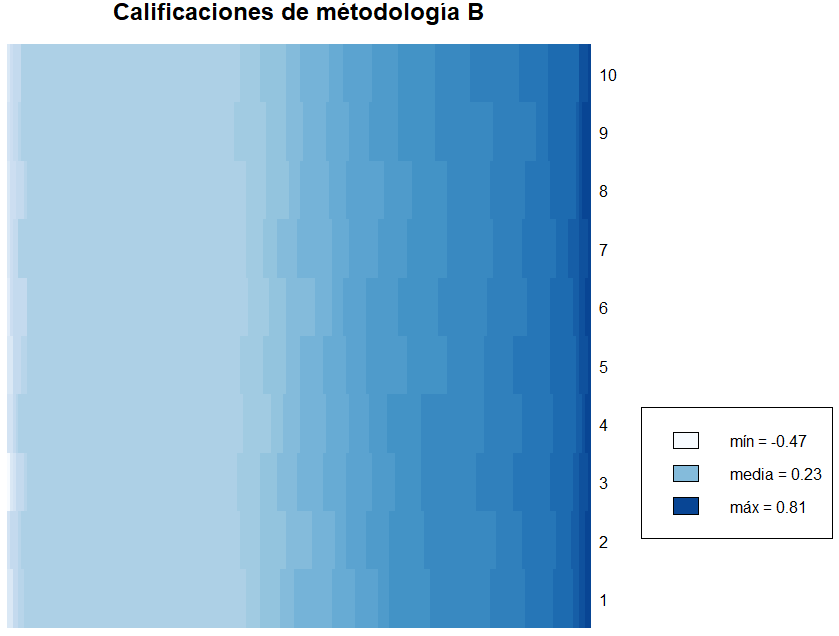
\includegraphics[scale = 0.5]{heatmap_metodo_B_2} %width=\textwidth
\caption[\textit{Heatmap metodología B}]{\textit{Se muestra el heatmap de las calificaciones por materia de la metodología B.}}\label{fig_heatmap_B}
\end{figure}

\begin{figure}[H]
\centering
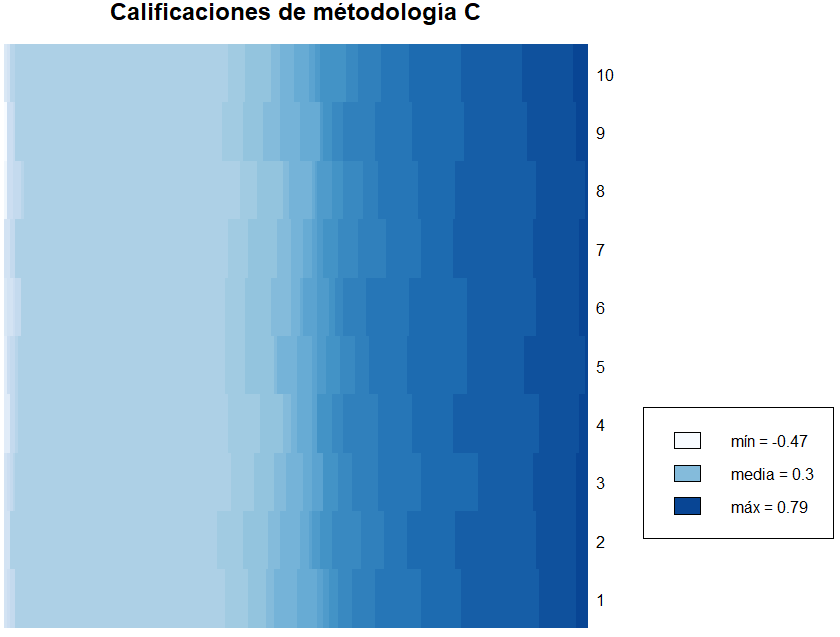
\includegraphics[scale = 0.5]{heatmap_metodo_C_2} %width=\textwidth
\caption[\textit{Heatmap metodología C}]{\textit{Se muestra el heatmap de las calificaciones por materia de la metodología C.}}\label{fig_heatmap_C}
\end{figure}


Para elegir entre las dos metodologías, tomamos en cuenta que el error relativo estuviera más cercano a cero. Al ver ambos \textit{heatmaps} observamos que el correspondiente al método $B$ es más claro que el del método $C$. Por lo que elegimos la metodología $B$ para simular los esqueletos. %En la siguiente sección explicaremos el procedimiento que seguimos para ésta metodología.

En la metodología $B$ la matriz $D'$ es una matriz \textit{mat\_demanda\_alumnos}. Es por ello que se genera con el procedimiento descrito en la Sección \ref{SimDemandaAlumnos}. La matriz \textit{mat\_esqueleto} se genera con el modelo de mezcla de Normales visto en la Sección \ref{sec_GMM}. En las siguientes secciones se describe a detalle el procedimiento que seguimos para obtener la matriz \textit{mat\_esqueleto}.

 %%Sección %%To include subfiles in to a subfiles use \input{name_of_file}

\section{Simulación de esqueletos} \label{sec_gen_esqueleto}

Para simular la matriz \textit{mat\_esqueleto}, con el modelo de mezcla de normales, necesitamos simular la información de varios esqueletos. Para ello vamos a considerar que ya se generaron las matrices $D'$ (ver Sección \ref{SimDemandaAlumnos}) y \textit{mat\_solicitudes} (ver Sección \ref{SimSolicitudesProfesores}). El proceso que seguimos para obtener un esqueleto es el siguiente:
  
  \begin{enumerate}
%\item Obtener la matriz \textit{mat\_demanda\_alumnos} con la demanda simulada del número de alumnos para el siguiente semestre (ver Sección \ref{GMM_D}).
%
%\item Obtener la matriz \textit{mat\_solicitudes} con las solicitudes simuladas de los profesores (ver Sección \ref{SimSolicitudesProfesores}).

\item Definir $num\_max\_asig = 2$, el número máximo de materias que pueden ser asignadas a un profesor.

\item Elegir un profesor de tiempo completo al azar.

\item Elegir al azar un horario y una materia que haya solicitado el profesor elegido en el paso anterior. Con estos datos obtenemos las coordenadas $(h,j)$ para las matrices $D'$ y \textit{mat\_esqueleto}.

\item Verificar que a esa materia en esa hora aún le sobran alumnos, en la entrada $(h,j)$ de $D'$.

\item Simular el número de alumnos para ese grupo (ver Sección \ref{SimTamGpos}).

\item Restar el número de alumnos simulados en el paso anterior, de la materia y hora elegidas, en la entrada $(h,j)$ de $D'$.

\item Ese profesor ya no puede impartir clases a esa hora. Retirar renglones respectivos de \textit{mat\_solicitudes}.

\item Si el profesor ya tiene $num\_max\_asig$ materias asignadas, eliminar la información del profesor de \textit{mat\_solicitudes}.

\item Repetir los pasos de 1 a 6 hasta que se terminen los profesores.

\item Una vez que se terminen los profesores de tiempo completo, hacer los pasos de 1 a 7 con los profesores de asignatura.
\end{enumerate}

Algunas notas a considerar del procedimiento son:
  
  \begin{itemize}
%\item[-] Se le da prioridad de asignación a los profesores de tiempo completo.

\item[-] Los profesores de tiempo completo deben cumplir con sus horas, por contrato.

\item[-] Los profesores sólo pueden tener asignadas a lo más $num\_max\_asig$ materias.

\item[-] Las condiciones de paro del proceso son:
  
  \begin{itemize}
\item[a)] Ya se cubrió toda la demanda

\item[b)] Ya no hay más profesores

\item[c)] Llegar a una cota predefinida para que el ciclo no se haga infinito o tarde mucho en cumplir las condiciones anteriores.
\end{itemize}
\end{itemize}


\section{Obtención de mat\_esqueleto} \label{sec_esqueletos}
%el Modelo de Mezcla Gaussiana visto en la sección \ref{sec_GMM}.

La matriz \textit{mat\_esqueleto} tiene $t$ renglones y $m$ columnas. En la entrada $(h,j)$ tiene el número de grupos simulados para la hora $h$ y la materia $j$. Dicha matriz depende de la demanda de alumnos y de las solicitudes de los profesores.


%Los pasos que seguimos para obtener la matriz \textit{mat\_esqueleto} con la metodología $B$ son:
Los pasos iniciales para obtener la matriz son:

\begin{enumerate}
\item Definir el número de veces que se va a generar la matriz $D'_{n}$ con la demanda de alumnos para el siguiente semestre, $n\_rep = 5$.

\item Simular $D'_{1}$ con la función \textit{gen\_mat\_demanda\_alumnos}. Los pasos de esta función se describen en la Sección \ref{SimDemandaAlumnos}.

\item Definir la matriz \textit{prom\_D} igual a $D'_{1}$. La matriz \textit{prom\_D} guardará el promedio del número de alumnos simulados.

\item Simular \textit{mat\_solicitudes} con la función \textit{gen\_solicitudes}. El procedimiento de esta función está descrito en la Sección \ref{SimSolicitudesProfesores}.

\item Simular un esqueleto inicial con la función \textit{gen\_esqueleto}. Los pasos de esta función se pueden ver en la Sección \ref{sec_gen_esqueleto}.

\item Guardar el número de grupos por materia.

\item Convertir y guardar los datos del esqueleto inicial para obtener la distribución por horas. Los datos se guardan en el vector \textit{wait\_mat\_esqueleto}.

\item Graficar los datos del esqueleto inicial para ver su distribución. Con esta gráfica encontrar el número de medias inicial, en nuestro caso $k = 4$ (ver \figurename{~\ref{hist_wait_esq_ini}}).

\begin{figure}[H]
\centering
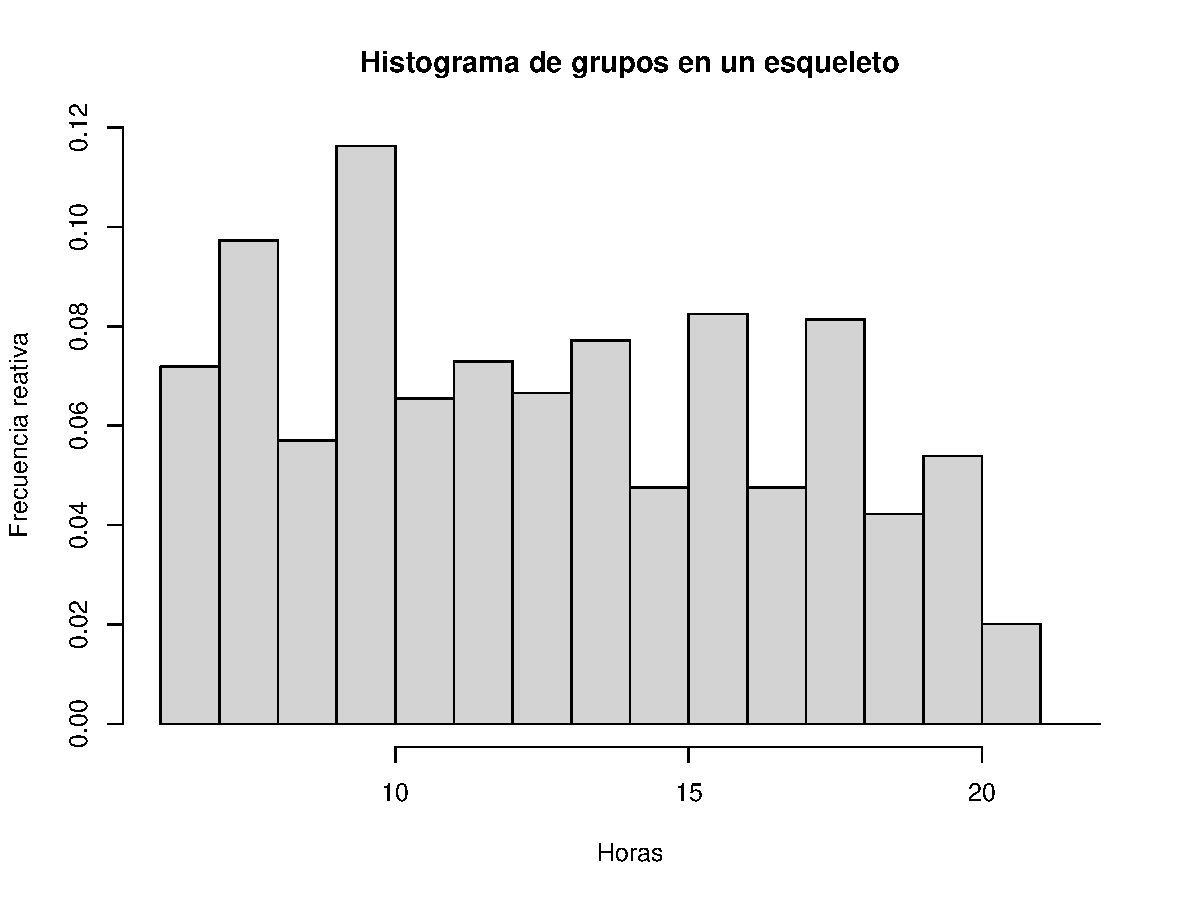
\includegraphics[scale = 0.7]{gmm_esqueleto_ini.pdf} %width=\textwidth
\caption[\textit{Histograma con los datos del esqueleto inicial}]{\textit{Se muestra el histograma con el número de grupos por hora en el esqueleto inicial.}}\label{hist_wait_esq_ini}
\end{figure}

\item Definir el modelo inicial \textit{mixmdl\_1\_esqueleto} con el siguiente comando en \textit{R}:

\verb@normalmixEM(wait_mat_esqueleto,k = 4)@.
\end{enumerate}

%\begin{figure}[H]
%\centering
%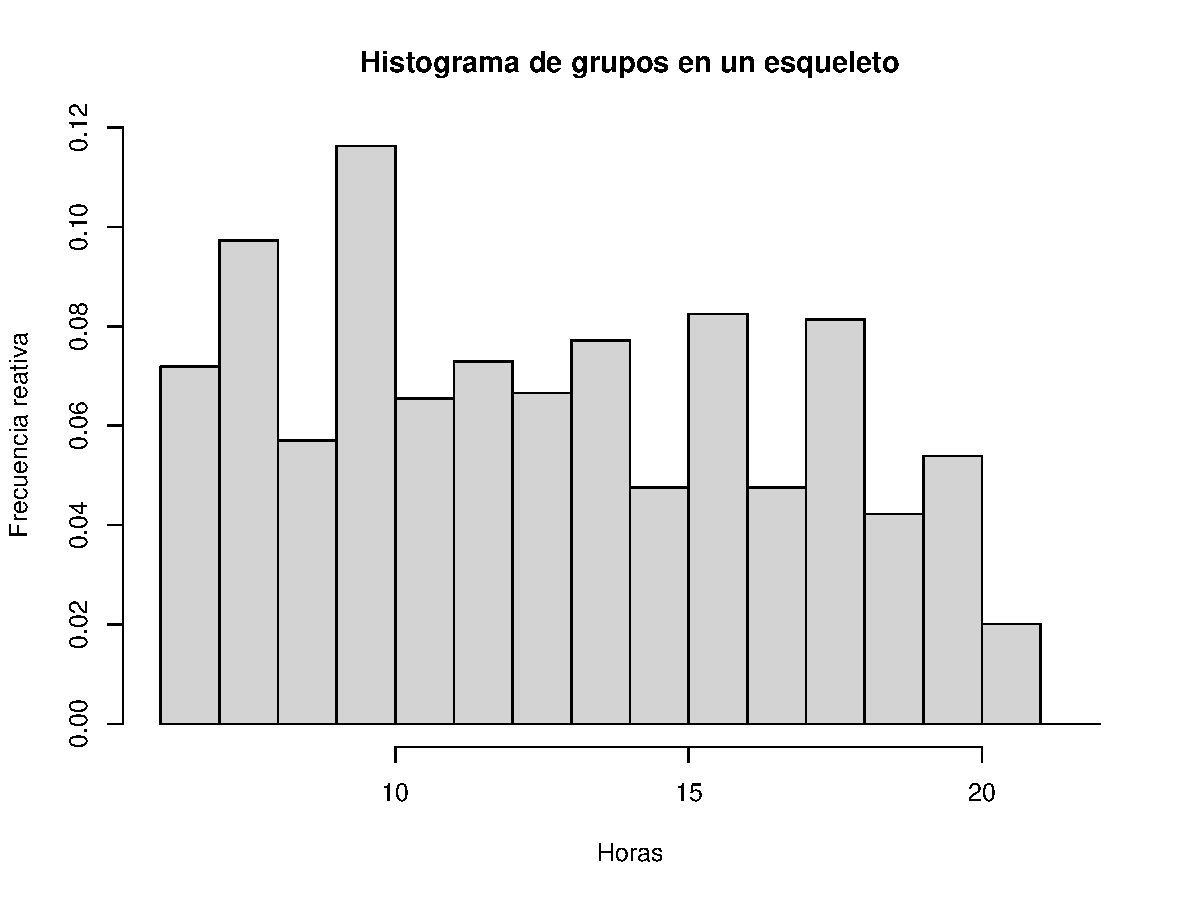
\includegraphics[scale = 0.7]{gmm_esqueleto_ini.pdf} %width=\textwidth
%\caption[\textit{Histograma con los datos del esqueleto inicial}]{\textit{Se muestra el histograma con el número de grupos por hora en el esqueleto inicial.}}\label{hist_wait_esq_ini}
%\end{figure}


Los pasos a repetir $(n = 2, \ldots, \textit{n\_rep})$ son:

\begin{enumerate}
\item Obtener $D'_{n}$ con la función \textit{gen\_mat\_demanda\_alumnos}.

\item Definir \textit{prom\_D} = \textit{prom\_D} + $D'_{n}$.

\item Simular \textit{mat\_solicitudes} con la función \textit{gen\_solicitudes}.

\item Simular un esqueleto con la función \textit{gen\_esqueleto}.

\item Guardar el número de grupos por materia.

\item Convertir y guardar los datos del esqueleto en el vector \textit{wait\_mat\_esqueleto}.
\end{enumerate}

Los pasos finales son:

\begin{enumerate}
\item Calcular el promedio de grupos por materia. Para ello, aplicar las siguientes funciones de \textit{R}, a la matriz \textit{prom\_D}: \verb@ceiling(colMeans((prom_D))@ 

\item Definir el modelo final \textit{mixmdl\_esqueleto}  con el siguiente comando en \textit{R}:

\verb@normalmixEM(wait_mat_esqueleto,k = 4,mean=mixmdl_1_esqueleto$mu)@.

En la \figurename{~\ref{hist_wait_esq_fin}}, se puede ver el histograma con todos los datos de los esqueletos simulados. La línea azul representa la distribución ajustada por el modelo final de mezcla de normales, \textit{mixmdl\_esqueleto}.

\item Generar la matriz \textit{mat\_esqueleto} en base al promedio obtenido y a la distribución del modelo final. Por ejemplo, si se tiene una materia con 5 grupos simulados, entonces se simulan 5 números aleatorios con distribución Normal. El comando en \textit{R} es: \verb@round(rnorm(5,mixmdl_esqueleto$mu,mixmdl_esqueleto$sigma))@
\end{enumerate}
 
\begin{figure}[h]
\centering
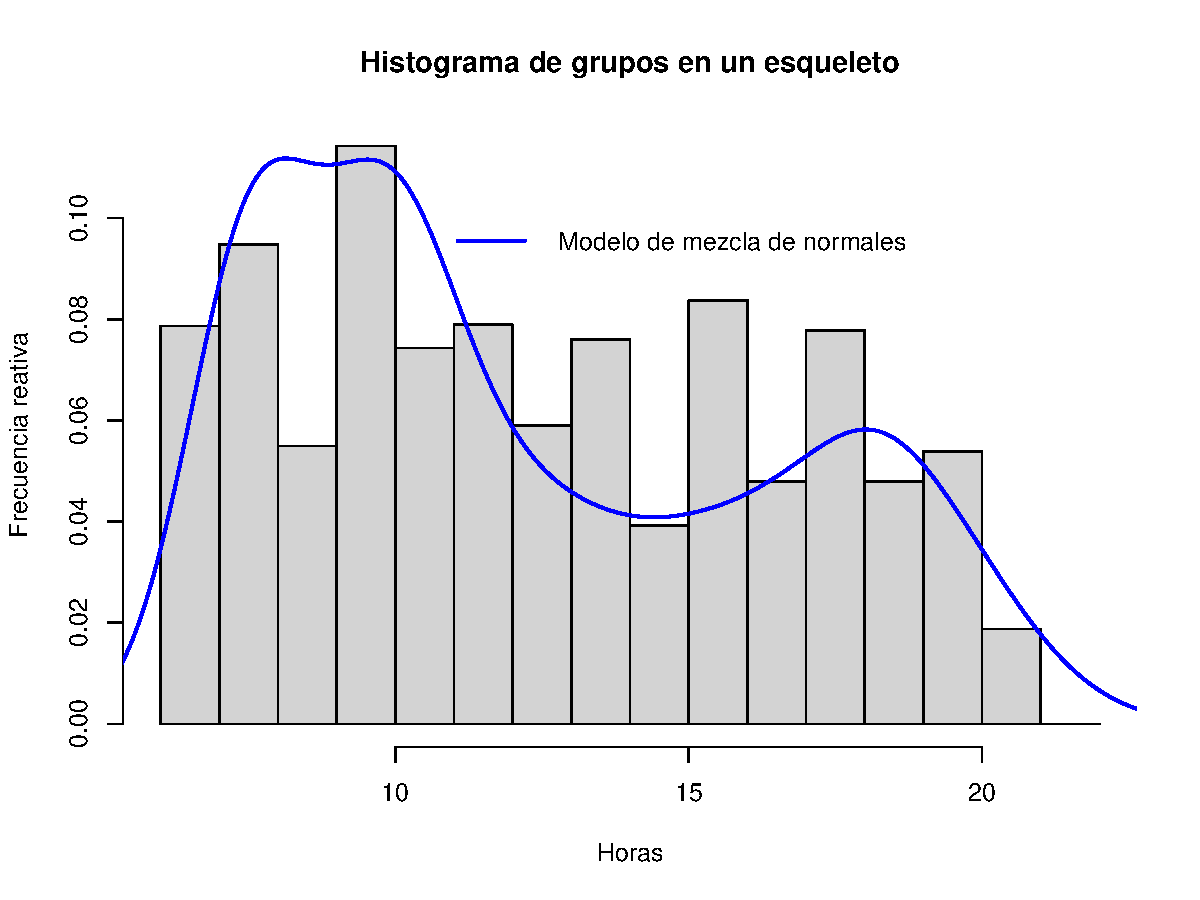
\includegraphics[scale = 0.7]{gmm_esqueleto_fin.pdf} %width=\textwidth
\caption[\textit{Histograma con  todos los datos de los esqueletos simulados}]{\textit{Se muestra el histograma con el número de grupos por hora de todos los esqueletos simulados. La línea azul representa la distribución ajustada por el modelo final.}}\label{hist_wait_esq_fin}
\end{figure}


En la \figurename{~\ref{esqueleto20202}} vemos un ejemplo de una submatriz de \textit{mat\_esqueleto} para el semestre 2020-2. Observemos las últimas 4 columnas que corresponden a las materias de \textit{Cálculo Diferencial e Integral I, II, III} y \textit{IV}.

Notamos que el número de grupos simulados para \textit{Cálculo Diferencial e Integral II} es mayor al número de grupos de \textit{Cálculo Diferencial e Integral I}. Ésto se debe al comportamiento descrito en la Sección \ref{Sec_AE_x_semestres} y el semestre 2020-2 es par. Para \textit{Cálculo Diferencial e Integral III} y \textit{IV} el número de grupos simulados es prácticamente igual.

\begin{figure}[H]
\centering
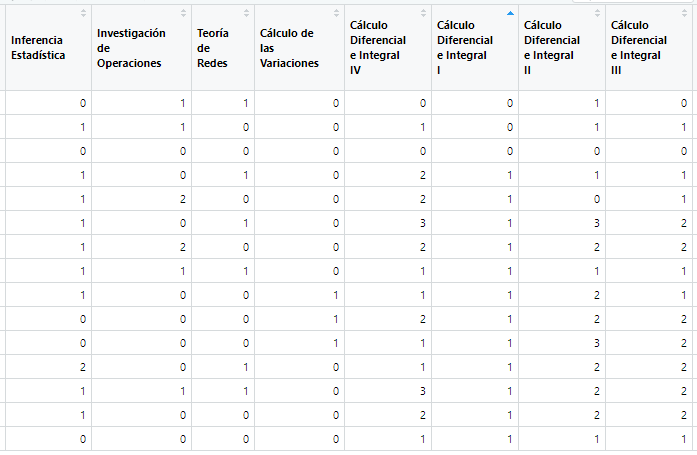
\includegraphics[width=\textwidth]{Ej_esqueleto_20202} %scale = 0.7
\caption[\textit{Esqueleto simulado para el semestre 2020-2}]{\textit{Se muestra una submatriz de ``mat\_esqueleto'' para el semestre 2020-2. En la entrada (h,j) se observa el número de alumnos simulados para la hora h y la materia j.}}\label{esqueleto20202}
\end{figure}


%\textbf{NOTAS:}
%
%\begin{itemize}
%\item[-] Sólo estamos haciendo operaciones cuando las entradas de \textit{bin\_DUE} haya un 1.\\
%
%\item[-] La diferencia relativa la definimos como $\dfrac{D - E}{D}$ porque la demanda es lo que esperamos que ocurra.
%\end{itemize}
%
%En la \figurename{~\ref{dif_D_E_gpo}} vemos el histograma de la diferencia de las matrices D - E. Diferencia entre el número de alumnos esperados menos el número de alumnos simulados por grupo. Los valores se encuentran entre -166 y 432.
%
%\begin{figure}[H]
%\centering
%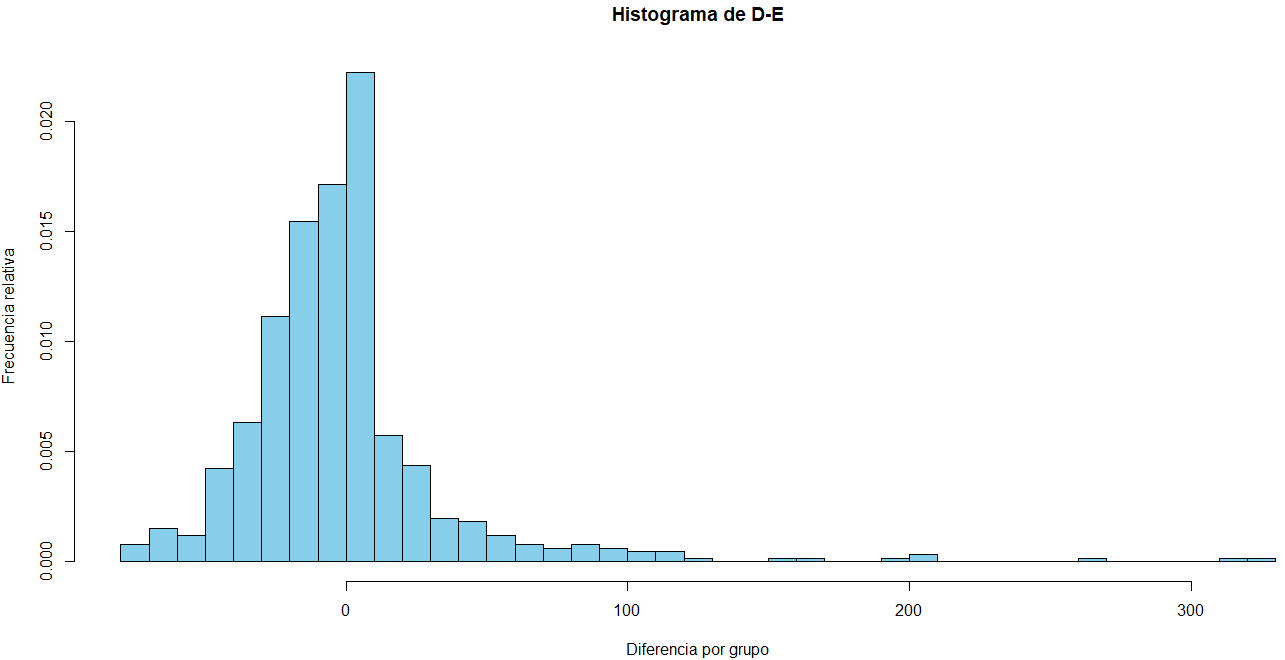
\includegraphics[scale = 0.5]{histograma_FR_D-E_x_gpo} %width=\textwidth
%\caption{\textit{Histograma de la diferencia de las matrices D - E por grupo}}\label{dif_D_E_gpo}
%\end{figure}
%
%
%En la \figurename{~\ref{difRel_D_E_gpo}} vemos el histograma de la diferencia relativa de las matrices D y E. Diferencia entre el número de alumnos esperados menos el número de alumnos simulados, entre el número de alumnos esperados, por grupo. Los valores se encuentran entre -71 y 1.
%
%El valor de -71 corresponde a la materia \textit{Teoría de los Conjuntos I}. A las 14hrs, en la matriz D vale 1 y en la matriz E vale 72 entonces el error relativo es -71.
%
%El valor de -64 corresponde a la materia \textit{Inferencia Estadística}. A las 12hrs, en la matriz D vale 1 y en la matriz E vale 65 entonces el error relativo es -64.
%
%El valor de -61 corresponde a la materia \textit{Probabilidad II}. A las 11hrs, en la matriz D vale 1 y en la matriz E vale 62 entonces el error relativo es -61.
%
%El valor de -61 corresponde a la materia \textit{Historia de las Matemáticas I}. A las 13hrs, en la matriz D vale 1 y en la matriz E vale 62 entonces el error relativo es -61.
%
%El valor de -50 corresponde a la materia \textit{Demografía}. A las 17hrs, en la matriz D vale 1 y en la matriz E vale 51 entonces el error relativo es -50.
%
%El valor de 1 corresponde a 111 materias, veamos 5 casos: \textit{Álgebra Moderna I (8hrs), Álgebra Lineal II (8hrs), Análisis Matemático II (16hrs), Manejo de Datos (16hrs), Seminario sobre enseñanza de las Matemáticas I (17hrs)}. En la matriz D valen 6, 16, 21, 3 y 7 respectivamente. En la matriz E valen 0, entonces el error relativo es 1.
%
%\begin{figure}[H]
%\centering
%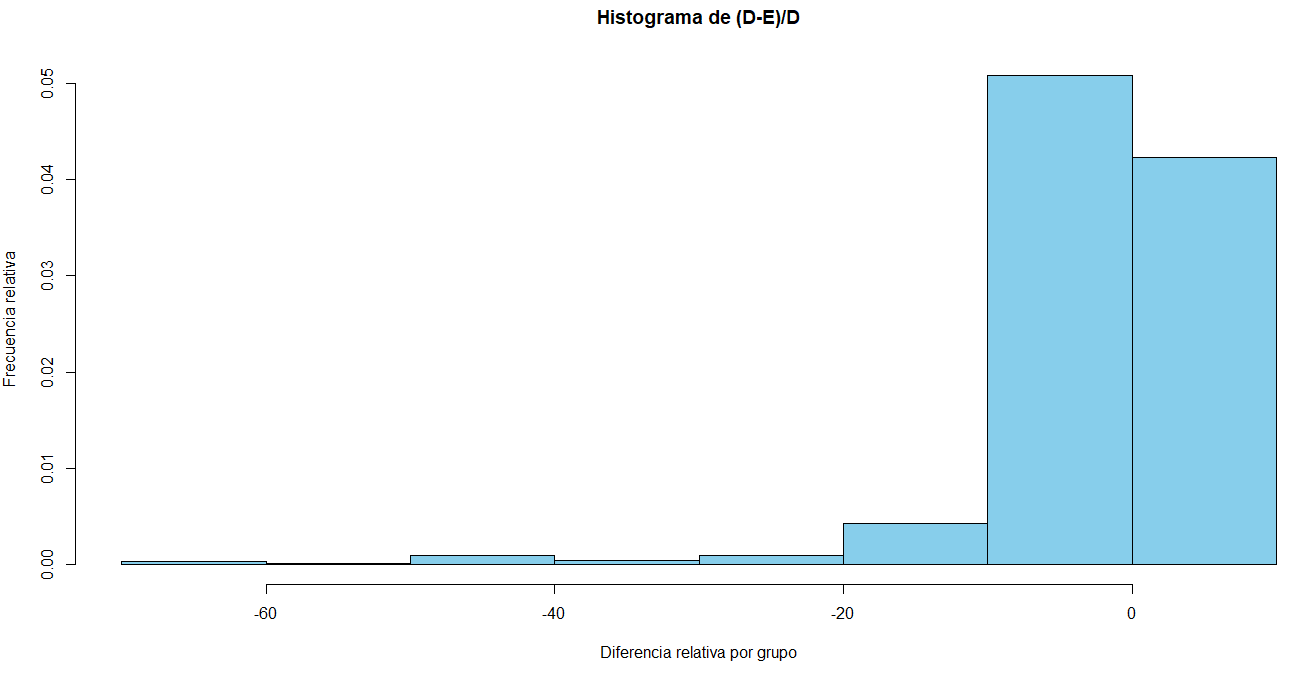
\includegraphics[scale = 0.5]{histograma_FR_D-E_D_x_gpo} %width=\textwidth
%\caption{\textit{Histograma de la diferencia relativa de las matrices D y E por grupo}}\label{difRel_D_E_gpo}
%\end{figure}


%En la \figurename{~\ref{dif_D_E_materia}} vemos el histograma de la diferencia de las matrices D - E. Diferencia entre el número de alumnos esperados menos el número de alumnos simulados por materia. Los valores se encuentran entre -259 y 244.
%
%\begin{figure}[H]
%\centering
%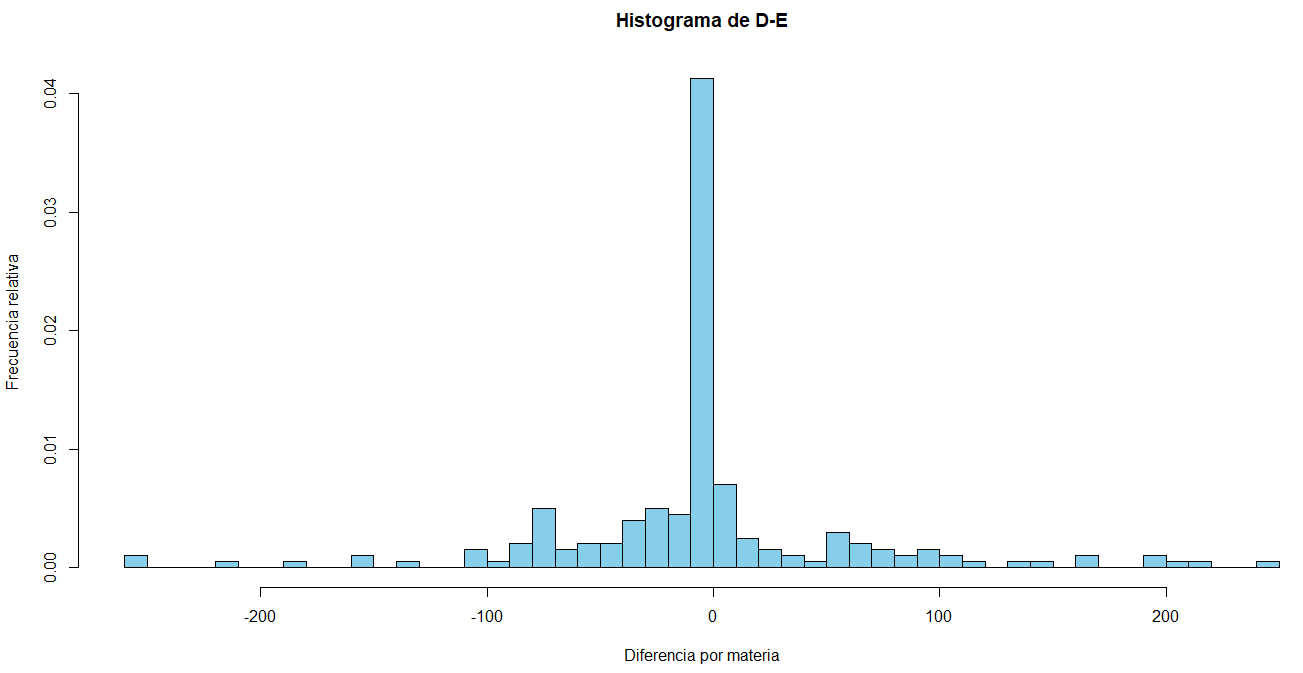
\includegraphics[scale = 0.4]{histograma_FR_D-E_x_materia} %width=\textwidth
%\caption{\textit{Histograma de la diferencia de las matrices D - E por materia}}\label{dif_D_E_materia}
%\end{figure}

%
%En la \figurename{~\ref{difRel_D_E_materia}} vemos el histograma de la diferencia relativa de las matrices D y E. Diferencia entre el número de alumnos esperados menos el número de alumnos simulados, entre el número de alumnos esperados, por grupo. Los valores se encuentran entre -97 y 6.
%
%\begin{figure}[H]
%\centering
%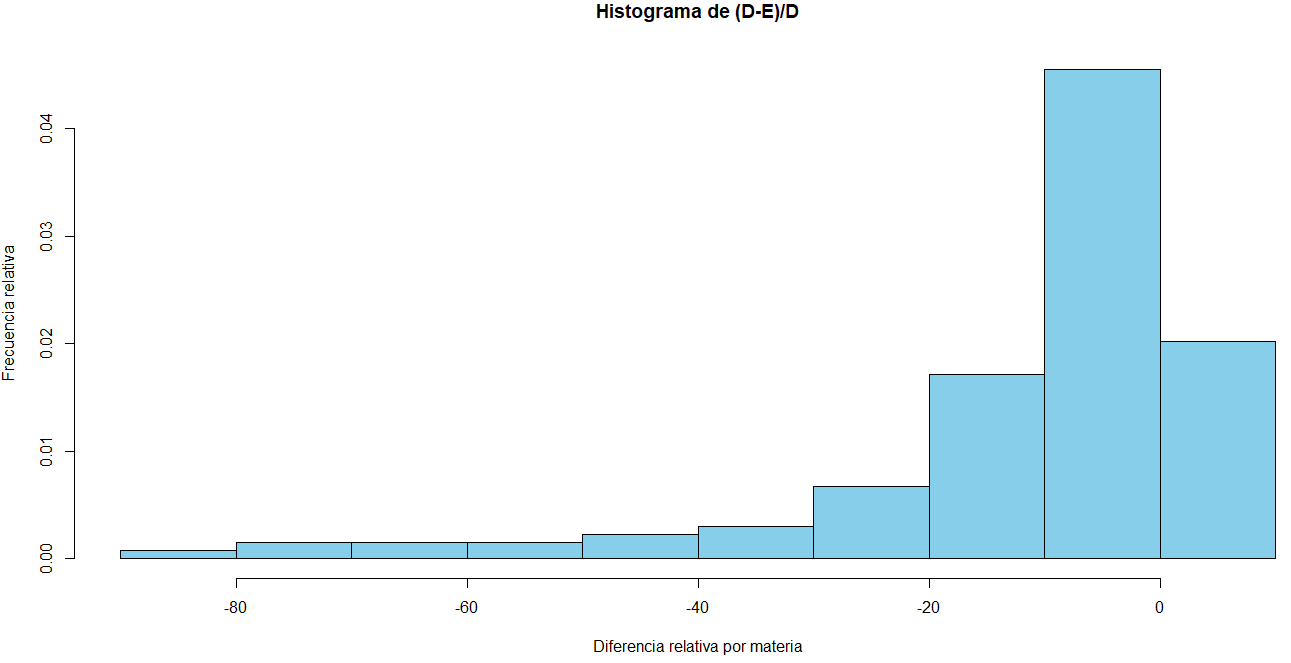
\includegraphics[scale = 0.4]{histograma_FR_D-E_D_x_materia} %width=\textwidth
%\caption{\textit{Histograma de la diferencia relativa de las matrices D y E por materia}}\label{difRel_D_E_materia}
%\end{figure}
%
%En la siguiente figura vemos las 20 materias con error relativo más negativo:
%
%\begin{figure}[H]
%\centering
%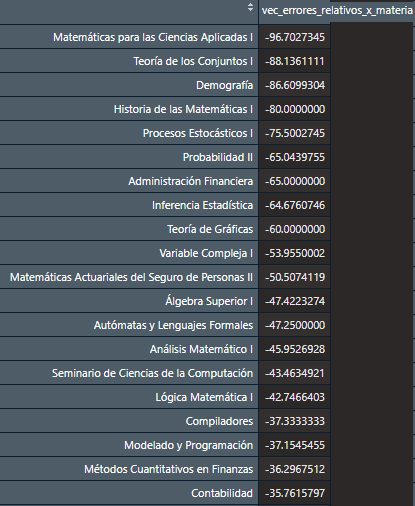
\includegraphics[scale = 1]{error_relativo_20materias_negativo} %width=\textwidth
%\caption{\textit{error relativo 40materias}}
%\end{figure}
%
%En la siguiente figura se tienen los valores en D y E de los 5 casos más negativos:
%
%\begin{figure}[H]
%\centering
%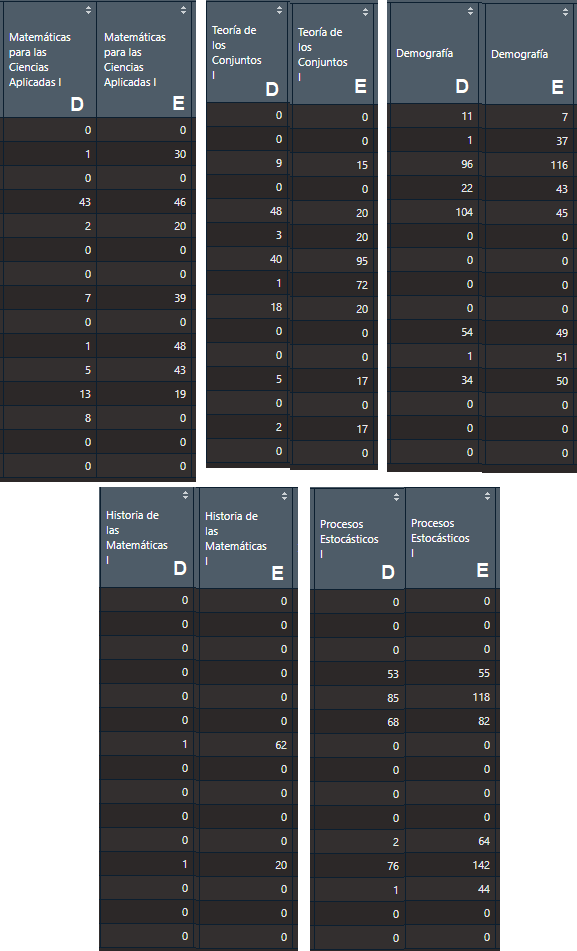
\includegraphics[scale = 0.85]{D_E_5_negativos} %width=\textwidth
%\caption{\textit{Casos más negativos}}
%\end{figure}
%
%
%En la siguiente figura vemos las 20 materias con error relativo más positivo:
%
%\begin{figure}[H]
%\centering
%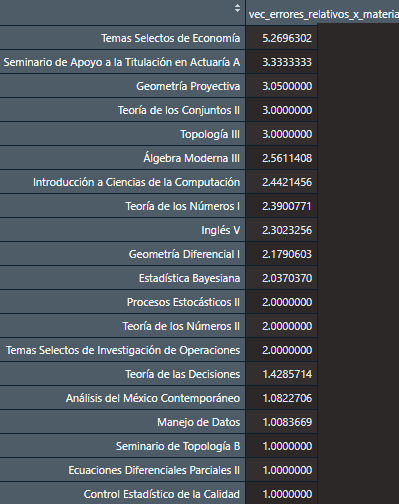
\includegraphics[scale = 1]{error_relativo_20materias_positivo} %width=\textwidth
%\caption{\textit{error relativo 40materias}}
%\end{figure}
%
%En la siguiente figura se tienen los valores en D y E de los 5 casos más positivos:
%
%\begin{figure}[H]
%\centering
%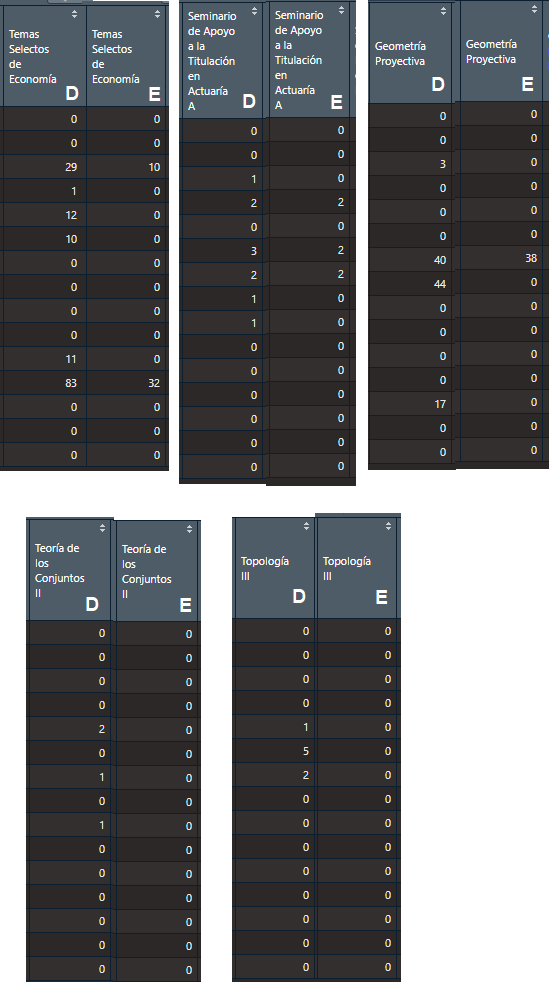
\includegraphics[scale = 0.9]{D_E_5_positivos} %width=\textwidth
%\caption{\textit{Casos más positivos}}
%\end{figure}
%
%
%\begin{eqnarray*}
%L_{materia} &=& -1 \,\,\,\,\,\,  \text{por cada materia no impartida}\\
%x &=& \text{promedio}\\
%y &=& \text{cupo}\\
%L_{dif\_p\_c} (x,y) &=& \begin{cases}
%\dfrac{a}{190} (x-y)  & \quad \text{si } x<y\\
%- \dfrac{b}{190} (x-y)  & \quad \text{si } x\geqslant y
%\end{cases}\\
%a &=& 0.5\\
%b &=& 0.8\\
%L_{categoria}^{1} (mat,solicitud) &=& -c(categoria - 1)\\
%L_{categoria}^{2} (mat,solicitud) &=& -c_{1}(categoria)
%\end{eqnarray*}
%
%Al momento de simular las solicitudes de materias para los profesores suponemos que la que está en primer lugar es la materia que más quiere dar, en segundo lugar, la segunda que quiere dar.
%
%Primero asignar grupos a los profesores de tiempo completo. Después asignar grupos faltantes a los profesores de asignatura.
%
%$L_{materia}$ es la penalización por no tener en el esqueleto una materia que necesitamos.
%
%$L_{dif\_p\_c}$ es la penalización en la asignación de salones. Se tiene un grupo de tamaño $x$ y un salón con capacidad $y$. Se penaliza con $\dfrac{a}{190}$ veces la diferencia entre $x$ y $y$ cuando el tamaño del grupo es menor a la capacidad del salón y se penaliza con $-\dfrac{b}{190}$ veces la diferencia entre $x$ y $y$ cuando el tamaño del grupo es mayor a la capacidad del salón.
%
%El esqueleto depende de la demanda de alumnos y de las solicitudes de los profesores.
%
%Primero se asignan materias a los profesores de tiempo completo y después a los de asignatura.
%
%Los profesores de asignatura pueden quedarse sin materias asignadas.
%
%Penalizaciones:
%  
%  \begin{enumerate}
%\item Si algún profesor pidió alguna materia y no se la dieron.
%
%\item Si hay alumnos que necesitan una clase a alguna hora y no existe profesor que la imparta.
%
%\item Con $\alpha \times num\_alumnos\_faltantes$ por cada alumno que te faltó en cada hora-materia que tenías que dar. $\alpha > 0$
%  
%  \item Con $\beta \times num\_alumnos\_sobrantes$ por cada alumno que te pasaste en cada hora-materia que tenías que dar. $\beta > 0$
%  
%  \end{enumerate}
%
%%Queremos el esqueleto con el menor valor en $\alpha + \beta$
%  
%  Con esto se califica un esqueleto.

